%
% Hosts Chapter
% Jason Brownlee
%
\chapter{Host Clonal Selection}
\label{chap:hosts}

%
% Overview
% Provides an overview of the chapter and its structure, and a description of what is intended to be achieved by providing this documentation. A description of why and how this chapter follows on from the previous chapter
%
\section{Chapter Overview}
\label{sec:hosts:overview}
This chapter extends the Tissue Paradigm, by raising the level of abstraction for clonal selection to that of a distributed population of self-governed immune systems interacting with each other in an antigenic environment. 
% background biology
Section~\ref{sec:hosts:biology} considers a holistic perspective of the mammalian immune system and reviews the ways in which populations of immune systems may interact with each other both directly and indirectly. Specifically, host immune system interactions are considered in the context of the passive and active forms of immunisation in a population and across generations, as well as the evolutionary concerns for the basis of immunological function.
% host paradigm
Section~\ref{sec:hosts:paradigm} abstracts the background biology of host immunisation and immune system evolution and presents the \emph{Host Clonal Selection Paradigm}. The paradigm is presented in terms of shared and evolved immunity interaction models, controlled and uncontrolled antigenic exposures, and population and generational host architectures. Collectively these concerns provide a foundation for the series of Host Clonal Selection Algorithms proposed and investigated in this chapter.
% population algorithms
Sections \ref{sec:hosts:population:elicited} and \ref{sec:hosts:population:shared} investigate the inter-population sharing of the trigger and product of acquired immunity respectively in a transmission and shared immunity algorithms. 
% generational algorithms
Sections \ref{sec:hosts:generational:maternal} and \ref{sec:hosts:generational:evolved} investigate the the inter-generational sharing of the product and the evolution of the mechanisms of acquired immunity respectively. 
% findings
The information processing and management strategies of the host paradigm demonstrated similar localisation and dissemination qualities as were demonstrated in the tissue paradigm with the additional level of control over interactions and decoupling of cellular repertoires promoted by the perspective of clonal selection.

%
% Populations of Immune Systems
%
\section{Populations of Interacting Immune Systems}
\label{sec:hosts:biology}
Immune systems do not exist in isolation, in terms of the various organs and interrelated subsystems within the host organism, or in terms of the populations to which the host organisms belong. In raising the level of abstraction to that of populations of immune systems, one may be interested in the manners in which immune systems interact. This transition may be considered as moving from thinking of the Darwinian struggle of lymphocytes within one host holistically providing a defence to the organism, to populations of these systems holistically providing a defence to a population (or a species). This section considers populations of immune systems, specifically with regard to evolutionary concerns and natural and artificial immunisation, and ways in which these systems may interact.  This general review is multi-disciplinary crossing such fields of study as population and evolutionary ecology, microbiology, epidemiology, and immunology. The intent of this section is to highlight some systems and processes that underlie the interactions between holistic immune systems to provide the basis for the inspiration of distributed computational Artificial Immune System models. 

%
% Immunisation
%
\subsection{Immunisation}
\label{sec:hosts:biology:immunisation}
Generally, immunisation implies that a host has been exposed to an antigen (immunogen) inducing an immune response that has educated the system with respect to more effectively and efficiently detecting and neutralising the antigen in the future. When a pathogen enters the host and elicits a response (and the host survives), the host gains a level of immunity to the pathogen. This process can be induced artificially through inoculation (controlled exposure to the pathogen), and is the basis of vaccination. Interestingly, immunity is not limited to this reactive method, and evolution has designed a temporary and passive form of immunity that is employed by mothers to protect children from pathogen before and after birth. This section reviews the various natural and artificial forms of acquiring immunity in terms of those mechanisms that elicit an immune response, and those that do not. Table~\ref{tab:hosts:immunisation:types} provides a summary of examples.

\begin{table}[ht]
	\centering\small
		\begin{tabular}{lll}
		\toprule
		  & \textbf{Natural} & \textbf{Artificial} \\ 
		\toprule
		\emph{Active}  & Infection & Vaccination, Inoculation \\ 
		\emph{Passive} & Maternal Immunity & Injection of antibodies \\ 
		\bottomrule
		\end{tabular}	
	\caption{Summary of the different types of immunity.}
	\label{tab:hosts:immunisation:types}
\end{table}

A developmental oddity of the acquired immune system is that the mass of the system is at its peak in early childhood, and decreases with time until early adulthood \cite{McDade1999}. This raises questions as to the usefulness of decreasing the resources of the defence system with age. An intuitive consideration would suggest that the size of the system would increase with the increase of acquired knowledge over the lifetime of the host. An answer to this question provides insight into acquired immunity as a strategy. Children are more vulnerable to infection than adults (children under the age of 5 suffer 8 to 24 times more infection than other age groups). Each pathogen encountered by an infant is novel and must be responded to anew. As a strategy, acquired immunity learns the hosts' pathogenic environment early and quickly. It provides an attempt to increase the hosts' early and prolonged survival within its environment. During the early stages of life the system maximises diversity, maximises cell proliferation potential, and maximises the rate of memory cell creation. Cell numbers peak in the first six months of life then steadily decline. Further, the developing infant immune system is buffered to the antigenic environment by the temporally inherited maternal immunity (natural passive) gained by the mother over her lifetime. This form of immunity is discussed in the following section.

%
% Passive Immunity
%
\subsubsection{Passive Immunity}
Passive immunity is the transfer of active humoral immunity in the form of ready-made antibodies to a host organism. Antibodies are relatively short-lived molecules that have no reproductive capability, thus the defensive capability provided by them is fast, effective, and temporary. A common form of natural passive immunity is maternal immunity (for review see \cite{Bienenstock1980, Englund1998, Hanson2003, Brandtzaeg2003}). Antibodies are provided by the mother to the foetus across the placenta and in breast-fed milk after birth (mucosal immunity). Vaccination of the mother during pregnancy may directly benefit the child as the antibodies produced by the mother will be passed to the foetus \cite{Glezen1999}. During breastfeeding, lymphocytes in the mother move to lymph nodes near the breast and release large amounts of antibodies into the breast milk. The antibodies enter the gut of the infant and provide protection against bacteria \cite{Slade1987}, and assists in oral tolerance (avoiding allergic reactions to food). The antibodies provide an initial and powerful boost in defence to the infant, which endures for a prolonged period after breastfeeding ceases. Breastfeeding stimulates the developing immune system, improving later response to vaccination, although initially suppresses the effector response of the infant immune system causing the failure of effective (artificial) vaccination during this period. It decreases infant mortality rate and provides benefits for the metabolism and disease resistance later in life \cite{Oddy2001}.

Passive immunity may be provided artificially through the transfer of blood or serum, and is applied when there is insufficient time for the host to develop an immune response. Some examples include viral and bacterial infections and poisons such as snake bites \cite{Keller2000}. Cell-mediated immunity may also be transferred in this manner (effector systems for detecting and neutralising infected cells rather than foreign molecules) and is called \emph{adoptive immunisation}. This is the transfer of recirculating lymphocytes rather than antibodies, although is difficult as such cells may be identified as foreign and attacked by the host immune system, thus the process is rarely used in humans. Monoclonal antibodies (mAb) are an artificial passive immunity where large quantities of identical antibodies are synthesised from identical cloned lymphocytes \cite{Vaughan1998}. Unlike polyclonal antibodies that vary in their specificity for an antigen, monoclonal antibodies all have the same specificity, and thus may provide a strong and directed defence. In theory it is possible to synthesise antibodies to recognise any substance. They are primarily used in biomedical research for detection and purification tasks, in the diagnosis of disease, and in the treatment of infections and cancer as delivery mechanisms \cite{Waldmann2003}. The process for producing monoclonal antibodies was first described in 1975 \cite{Kohler1975}, and later refined for human use \cite{Riechmann1988}.

%
% Active Immunity
%
\subsubsection{Active Immunity}
Active immunity involves the stimulation of the system by an antigen and the development of an immune response. Natural active immunity is the normal functioning of the acquired immune system for neutralising pathogens. Artificial active immunity involves intentionally inducing the immune response by introducing an immunogen in a vaccine. A vaccine is typically administered before the patient contracts the disease, although it may be administered after, assuming the immune response to the immunogen is faster than the response to the infection. There are many different types of vaccines including inactivated (dead) pathogens, live attenuated (low virulence) pathogens, toxoids (inactive toxic compounds from pathogens), and subunit or pieces of pathogens. Vaccination does not prevent the host from contracting the disease, rather like natural active immunity it provides an improved response to the disease making it harder for it to spread throughout the population. Vaccination is one of the greatest achievements in medicine and public health \cite{Salmon2006}. The ethics of compulsory vaccination are still debated throughout the world, although the benefits of immunity to disease and disease eradication are generally considered to outweigh the costs of a minority of recipients contracting the disease the vaccine was designed to prevent. An aspect of population vaccination is an effect called \emph{herd immunity} \cite{Fine1993, Anderson1985, Anderson1990}. This is where the majority of the population (perhaps more than 90\%) is vaccinated for a disease, which provides protective coverage for the entire population. An impact of this interesting effect is that vaccination schemes may not be concerned with immunising the remainder of the un-vaccinated population, rather the immunisation of enough of the population to reduce the chance (to a desired level) of a member of the population contracting the disease.

%
% Evolution
%
\subsection{Evolution}
\label{sec:hosts:biology:evolution}
The acquired immune system of mammals (such as humans, mice, rats, and cattle) is the most studied immune system. A consideration of the system in the context of the `tree of life' reveals that this it belongs to a very small minority of taxa: the jawed vertebrates, raising the question as to why this system evolved when all other plants and animals survive without it. Evolution has designed a complex, specialised, and multi-layered defence in the immune system \cite{Danilova2006}, although the system is not perfect: \emph{``\ldots vertebrates are exquisitely adapted [\ldots] but not perfectly; autoimmunity and cancers present the costs and failures of immunity''} \cite{Rinkevich2004} (page 33). The very fact that mammals are vulnerable to disease highlights that the immune system is a sub-optimal adaptation \cite{Nesse2005}. Interestingly, some suggest the acquired immune system may be an evolutionary misstep given all the positive and negative feedback signals (checks and balances) needed to regulate an immune response \cite{Hedrick2004}.
% section
This section provides a brief review of the innate and acquired immune systems from an evolutionary perspective. 

%
% The Innate and Acquired Immune Systems
%
\subsubsection{The Innate and Acquired Immune Systems}
The innate immune system is a collection of defence mechanisms, tissues, and specialised processes that defend the host from its pathogenic environment. The innate defence is inherited and defined in the genome, thus the specificity for the pathogens it may detect is `hard-wired' throughout the hosts lifetime. The trade-off for this rigidity is that the defence it provides is fast, practically instantaneous. In the acquired immune system, evolution has designed a somatic learning system that may recognise any biochemical molecule, although this tool of defence may also destroy the host which it is intended to protect. Acquired immunity is a personalised defence, learned within the context of the hosts' specific pathogenic environment. It is slow acting, requiring an aggregation of antigen encounters generally over about a week before it is ready to fight the pathogen (fast compared to the innate system which specialised over generational time). As a strategy, the system is anticipatory, assuming that future pathogenic encounters will be the same or similar to past pathogenic encounters. Table~\ref{tab:hosts:evolution:innateacquired} contrasts some of the properties of the acquired and innate immune systems.

\begin{table}[ht]
	\centering\small
		\begin{tabular}{lll}
		\toprule
		\textbf{Receptor's Features} & \multicolumn{2}{c}{\textbf{Immunity Systems}} \\ 
		\midrule
		 & \textbf{Innate} & \textbf{Adaptive} \\ 
		\toprule
		\emph{Distribution in cell populations} & uniform & clonal \\ 
		\emph{Specificity} & low & high \\ 
		\emph{Affinity} & $10^3-10^4$ & $10^6-10^{11}$ \\ 
		\emph{Diversity (the number of variants)} & $10^2-10^3$ & $10^9-10^{11}$ \\ 
		\emph{Variability} & absent & high \\ 
		\emph{Ligand origination} & foreign (non-self) & foreign and self \\ 
		\bottomrule
		\end{tabular}
	\caption{Summary of the differences between the innate and acquired immune systems, taken from \cite{Klimovich2002} (page 565).}
	\label{tab:hosts:evolution:innateacquired}
\end{table}

The acquired immune system is exceedingly complex, such that approximately 5\% of the genome of humans is proposed to be for molecules used in the system. This antibody immunity is proposed to have evolved gradually over a long period of time from cells and tissues that previously performed other functions \cite{Klein2005}. Klimovich considers some of the problems related to the evolution of the acquired immune system highlighting: (1) the system was formed in the presence not only of pathogen but also coexisting foreign organisms living in symbiosis, (2) many kinds of activity in the system are not protective in nature, instead serving alternate functions, and (3) the system performs the learning function \emph{before} applying the protective mechanism (so called pre-committed) \cite{Klimovich2002}. Hedrick suggests that perhaps long-lived complex jawed vertebrates need an acquired immune system, highlighting that the acquired immune system may be an approximate solution to the problem of parasitism, providing a small advantage in reproductive success that invertebrates could not afford the cost of resources to evolve, maintain, and exploit \cite{Hedrick2004}.


%
% Summary
%
\subsection{Summary}
\label{sec:hosts:biology:summary}
The evolution of immunity is the interaction of immune systems both with their environment, which may be adversarial in the case of parasites, and with each other in terms of reproduction and natural selection. Sexual recombination of the genetics of immunity provides interactions of immune systems in terms of new arrangements of existent traits. The pressure of natural selection results in the implicit competition between heterogeneous populations of immune systems in a spatial-temporal pathogenic environment. Immunisation provides a second example of the interaction between immune systems. Evolution designed the mammalian acquired immune system to be augmented in infancy by the lifetime immunological knowledge of the maternal immune system in a temporary Lamarckian-style inheritance. This natural passive immunity provides a robust replacement defence for the developing system. Additionally this process may be reproduced artificially later in life by the removal of antibodies from one host and then injected into another to provide a short-lasting immediate defence to a pathogen.

%
% Host Paradigm
%
\section{Abstract Host Paradigm}
\label{sec:hosts:paradigm}
% the paradigm
This section abstracts and elaborates on a host-centric adaptive strategy and proposes a \emph{Host Clonal Selection Paradigm} that takes the Tissue Paradigm and implicitly the Cellular Paradigm for granted, and focuses on the inter-host interaction and information sharing provided by bottom-up host-population and host-generational immunisation and evolutionary mechanisms. Conceptually, a \emph{host} represents a rise in the level of abstraction from a \emph{tissue} (conventional clonal selection algorithm or repertoire) to a collection of such tissues working together to provide holistic immunological function. Therefore a \emph{Host Clonal Selection Algorithm} is concerned with a system comprised of a number of \emph{Tissue Clonal Selection Algorithms} (Chapter \ref{chap:tissues}) that in effect are the components or units of adaptation (hosts) within a host algorithm.

%
% Model Components
%
\subsection{Interaction Models}
\label{sec:hosts:paradigm:interaction}
The host paradigm is primarily concerned with the interaction of whole immune systems where the considerations of what happens within a single host is delegated to the Tissue Paradigm, and in turn the Cellular Paradigm for the concerns within a single tissue repertoire of cells. This section considered the two primary means in which immune systems can interact and more importantly effect each other: \emph{explicitly} and \emph{implicitly}. Explicit interaction between host immune systems is defined as \emph{Effector Sharing} where the information acquired by an immune system (its effectors) are shared with other immune systems either by passive infusion or active response elicitation. Implicit interaction between hosts involves evolutionary processes over generational time that effect the basis and processes by which progeny immune systems acquire information called \emph{Evolved Immunity}.

%
% Effector Sharing
%
\subsubsection{Effector Sharing}
\label{sec:hosts:paradigm:interaction:sharing}
Immunity is acquired and refined over the lifetime of the host given antigen exposures and resultant clonal selection and affinity maturation. The effectors produced in this process (antibodies, memory and recirculating lymphocytes) may be shared with other immune systems. In this context \emph{effector} is a generalised term that refers to some discrete information acquired by an immune system such as the product of a clonal selection and expansion event. This section describes two mechanisms for sharing effectors between systems in what is referred to as passive immunity: \emph{Vertical Sharing} and \emph{Horizontal Sharing}. 

%\begin{figure}[ht]
%	\subfloat[Vertical Effector Sharing.]{
%	\label{fig:hosts:paradigm:sharing:vertical} %% label for first subfigure
%	\begin{minipage}[c]{0.5\textwidth}
%		\centering 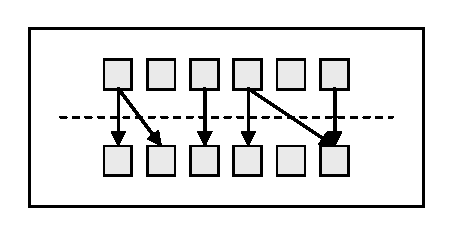
\includegraphics[scale=0.85]{Hosts/hosts-sharing-vertical}
%	\end{minipage}}%
%	\hfill
%	\subfloat[Horizontal Effector Sharing.]{
%	\label{fig:hosts:paradigm:sharing:horizontal} %% label for second subfigure
%	\begin{minipage}[c]{0.5\textwidth}
%		\centering 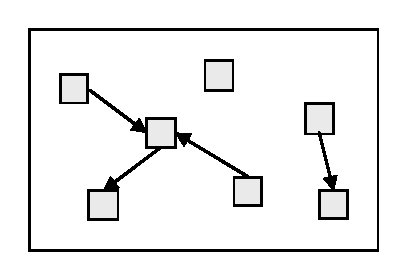
\includegraphics[scale=0.70]{Hosts/hosts-sharing-horizontal}
%	\end{minipage}}
%	\caption{Depiction of vertical and horizontal effector sharing.}
%	\label{fig:hosts:paradigm:sharing} %% label for entire figure
%\end{figure}

\paragraph{Vertical Sharing}
Vertical sharing is inspired by natural passive immunity such as the sharing of antibodies between mother and foetus across the placenta (maternal immunity), and to the infant after birth through breastfeeding (mucosal immunity). Vertical sharing of immune effectors is a mechanism of inheriting acquired immunity between generations. A sample of the effectors are removed from a parent system and inserted into a child system. The shared effectors, such as all cellular components have a finite lifetime and may perish before being employed by the receiving system. A natural version of this mechanism is a parent-child relationship, but this is not a requirement. The mechanism does require (1) a generational population structure, (2) the selection of a donor from the previous generation, (3) the selection of a receiver from the next generation, and (4) a sampling method for the donor (effector selection mechanism).	
 
\paragraph{Horizontal Sharing}
Horizontal sharing of immunity effectors is inspired by artificial passive immunity where effectors are synthesised and injected into hosts, or removed from one host and injected into another. This method of effector sharing provides a way of transferring learned immunity within a population of immune systems. The mechanism does not require a generational population structure, although, like vertical sharing it does require (1) a donor of effectors (within the population or synthesised externally), (2) a receiver system within the population, and (3) a sampling (selection) method for effector cellular components from the donor.

%
% Evolved Immunity
%
\subsubsection{Evolved Immunity}
\label{sec:hosts:paradigm:interaction:evolution}
Another way of sharing immunity is through genetic evolution involving (1) the assignment of immune system fitness, (2) selection of parent immune systems, (3) the recombination of parent genetic material to create children, and (4) the mutation of child genetic material. Those immune systems that demonstrate their relative utility (relative to other immune systems with the same generational population) may proliferate, and those that do not demonstrate utility, perish. The evolution of immune systems requires that the expressed phenotype (thing being evolved such as immune effectors or response strategy) be transcribed from a genome (representation) on which the evolutionary processes of selection, recombination, and mutation may operate. It requires a generational mechanism for implicitly sharing effectors (seed and process for creating effectors) rather than explicitly as in the case of vertical and horizontal effector sharing. Two evolved immunity mechanisms are presented as follows: (1) Evolution of an Innate Immunity, and (2) Evolution of an Acquired Immunity.

\paragraph{Innate Immunity}
Innate immunity may be thought of as hard-wired defence mechanisms that are learned in response to pathogens within a species over generational time. A simple example is a static recognition and response rule system for a host, which although remains fixed for the lifetime of a single host, evolves to protect the whole species. In this example, the rule system is fast acting on the lifetime scale, although slow to change on the same scale implying perhaps the increased expendability of individuals for the greater good of the species.	

\paragraph{Acquired Immunity}
The acquired immune system, although is a somatic learning system rapidly adapting to the hosts pathogenic environment, may also acquire more generalised species level traits via evolution. Evolution may be used to evolve the acquired immune system by biasing the creation of \naive\ lymphocytes to specific sub-areas of the shape-space. This bias may accelerate the acquisition of immunity by individuals, requiring less work by the somatic learning system.	


%
% Antigenic Exposures
%
\subsection{Antigenic Exposures}
\label{sec:hosts:paradigm:exposures}

%
% Discrete Host Exposures
%
\subsubsection{Discrete Host Exposures}
\label{sec:hosts:paradigm:exposures:discrete}
Section~\ref{subsubsec:tissues:paradigm:exposures:discrete} extended the \emph{Antigenic Exposure Paradigm} of Section~\ref{subsec:cells:paradigm:antigenicexposures} to include the notion of multiple points of exposure on a Tissue Clonal Selection Algorithm (each repertoire). The attributes of discrete exposure were bundled into a concept called the \emph{Tissue Exposure Pattern}. This concept was specialised to incorporate spatial and temporal regularities of exposure location and duration in order to assess the information acquisition and dissemination properties of tissue models called an \emph{Antigenic Infection}. The aggregation of multiple antigenic infections on a tissue was referred to as situating the tissue model (host) in an \emph{Antigenic Habitat}. Like Tissue Clonal Selection Algorithms, Host Algorithms also provide multiple points of exposure in an antigenic environment and therefore have similar concerns. Figure~\ref{fig:hosts:paradigm:exposure:spatial} provides a conceptualisation of a spatial population of discrete hosts, each situated in their own antigenic habitat.

% Classical spatial picture of exposing multiple systems
\begin{figure}[ht]
	\centering	
	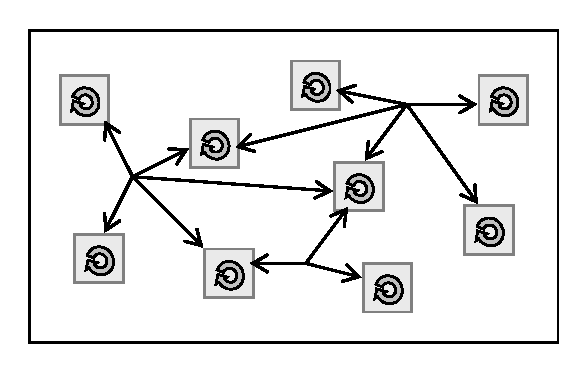
\includegraphics[scale=0.85]{Hosts/hosts-exposure-spatial}
	\caption{Host Clonal Selection Model and the situated spatial properties that affect antigenic exposure, where the arrows represent interaction between the discrete components (hosts) in the system.}
	\label{fig:hosts:paradigm:exposure:spatial}
\end{figure}

% differences between hosts and tissues, introduction of env
There are two distinct and important differences between the Tissue and Host paradigms with regard to antigenic exposures: (1) exposures of antigen to hosts may be both controlled (elicited by other hosts) and uncontrolled (environmental) whereas tissue models have no control over such exposures, and (2) the level of abstraction regarding exposures is raised from that of an habitat of infections for a single host, to multiple and potentially different (asymmetric) habitats across multiple hosts called an \emph{Antigenic Environment}. 

%
% Controlled and Uncontrolled Exposures
%
\subsubsection{Controlled and Uncontrolled Exposures}
\label{sec:hosts:paradigm:exposures:control}
The acquired immune system learns through exposure, detection, and response to antigens, thus the antigenic environment defines what is learned and when. The immunity that a system receives through recognising and responding to antigens is called active immunity and may be induced naturally (uncontrolled) and artificially (controlled). 

\paragraph{Uncontrolled Exposure}
Uncontrolled antigen exposure is a natural way for a system to achieve active response-based immunity. This form of antigen exposure is an elaboration of the previously defined standard model. An aspect of the distinctiveness of acquired immune systems in a population is the spatial and temporal variations of antigen exposures. These varied exposure patterns in conjunction with the varied \naive\ repertoire of each individual result in distinct initial and learned specificities to antigens. For a given antigen, exposure may be described as a function over space and time that may be skewed for many reasons such as antigen virulence, host density, and other pathogen-behaviour and spatial-population effects.

\paragraph{Controlled Exposure}
Control over antigen exposure provides control over immunity of individual systems and virtual immunity over the entire population through effects like `herd immunity'. Artificial exposure of systems to antigen provides control of (1) which systems are exposed to (2) what antigen (3) when. A vaccination exposure strategy may involve administering a vaccine to a large number of systems quickly. An inoculation strategy may involve exposing a select few systems to the antigen in a short amount of time. Control of exposures may also extend to preventative steps such as environment sterilisation or individual system isolation from the antigenic environment.



%
% Antigenic Habitats and Environments
%
\subsubsection{Antigenic Habitats and Environments}
\label{sec:hosts:paradigm:exposures:habitats}
The Tissue Exposure Regime of the Tissue Paradigm may be extended to a \emph{Host Exposure Regime (HER)} that defines which hosts are exposed to antigen and when they are exposed. This means that the system is less concerned with how well a given host can specialise a response and internally disseminate acquired information, and more concerned with how that information is acquired and disseminated between hosts in the population. Unlike tissues, hosts are not restricted to fixed network topologies like the ring network structure of the Lymphocyte Recirculation Algorithm, therefore asymmetries in the Host Exposure Regime and the host interaction patterns define the capability and speed of information dissemination throughout the population. 
% Pathogenic Environment
Given the shift in focus from the internal process of information acquisition within a host to the internal information acquisition of a population of hosts, the antigenic environment may be conceptualised as a \emph{Pathogenic Environment} consisting primarily of exogenous antigen. This does not mean hosts may not respond and communicate information regarding endogenous antigen, rather it suggests that the focus of the Host Paradigm is hosts and their relationships with external antigen that may come the environment and other hosts.
% pathogen as an entity
In addition to the Host Exposure Regime, the rise in the level of abstraction in the Host Paradigm facilitates broader concepts regarding antigen as self-contained entities, in particular (1) the co-evolution of pathogen with a population of hosts, and (2) the contraction of a pathogen by a host and transmission to neighbouring hosts. 

\paragraph{Evolvable Pathogen}
A pathogen may explicitly evolve or co-evolve with the population of immune systems. Evolution may refine the strategy of the pathogen affecting configuration such as virulence and transmissibility. An individual acquired immune system may be open to multiple infections by the same pathogen during its lifetime if the rate of evolution is sufficiently rapid. Such a pathogen may require tracking and ultimately evolving countermeasures by the host population, perhaps facilitating a host-parasite interaction.

\paragraph{Transmittable Pathogen}
After exposure to a host, a pathogen may jump from host-to-host using a number of mechanisms (vectors). Further, transmissibility may be influenced by any number of epidemic-based host models such as density-dependence, spatial models, and genetic-similarity models.	

%
% Host Architectures
%
\subsection{Host Architectures}
\label{sec:hosts:paradigm:architectures}
The abstraction of immune system interaction models of immunisation and evolution suggests two distinct Host architectures as follows: (1) \emph{Populations of Hosts} that focus on the natural and artificial elicitation of immune response and transfer of acquired immunity, and (2) \emph{Generations of Populations of Hosts} that focus on hosts with a finite life-cycle that include inter-generational elicitation and transfer of immunity and the evolutionary change of the properties of lifetime innate and acquired immunity. This section outlines these two distinct host architectures.

%
% Population Model
%
\subsubsection{Population Host Model}
% Host Population Model
An acquired immune system does not exist in isolation, rather it is a collection of organs and tissues that collectively represent an integrated part of a host organism, which in turn belongs to a population of such organisms. One may consider the hosts of a population interacting with each other, more specifically interacting with regard to their immune systems. The class of model in which a population of clonal selection-based immune systems interact with each other is referred to as a \emph{Population Host Model}. The focus of this model is the host as the unit of adaptation, each with a distinct starting point, and likely distinct antigenic environment including interactions with the environment and other hosts. This diversity provides robustness in the population with regard to information acquisition and dissemination, abstracting concerns of population survivability in an unknown environment. 
% making the case for interactions within a population
A population of non-interacting hosts facilitate the development of multiple varied perspectives of an antigenic environment that remain isolated. Integration of this information without host interaction mechanisms would require augmentation from a higher level of abstraction (the population level). The \emph{isolated perspectives} property of the population model is made more apparent in an asymmetrical pathogenic environment. In such an environment, not only does the heterogeneous population acquire information in different ways and rates, but the information content of the environment to which they are exposed also varies. Therefore, although the population may collectively represent a map of the environment, there is no way for individual systems to share acquired information. This concern is further highlighted if we consider that the asymmetrical pathogenic exposure regimes for the systems in the population vary over time. In this case, the information acquired by one system is directly useful to other systems, although cannot be exploited. 
% case for extension - all about balancing specialisation with dissemination
A population of non-interacting hosts provides a foundation on which to incorporate intra-population (inter-host) interactions. Intra-population re-transmission of captured antigen, and intra-population effector sharing provide two examples that motivate the investigation of decentralised intra-population interactions.

%
% Generational Model
%
\subsubsection{Generational Model}
% Host Generational Model
Host organisms in a population reproduce such that a generational structure may be defined between hosts where progenitor-hosts produce progeny-hosts. In this mechanism, the population of immune systems (the present generation) are responsible for creating a new set of immune systems (the next generation), which replace members of the present generation. This principle defines the \emph{Generational Host Model} that provides an extension to the proposed Host Population Model. Hosts may use an asexual reproduction mechanism where one host contributes a variation of itself to the next generation. Alternatively, hosts may collaborate in their contributions to successive generations (sexual reproduction). Further, the contributions of various hosts to successive generations may not be homogeneous, such that more successful hosts (by some measure of success) may contribute more than less successful hosts.
% components
The principle components of the generational approach are (1) the reproductive scheme, and (2) the mechanism that triggers the generational change.

\begin{itemize}
	\item \emph{Reproductive Scheme}: The mechanism by which one generation contributes to and prepares the successive generation. Examples include sexual and asexual reproduction where hosts may or may not cooperate in their contributions to the next generation. Further, the contributions of any one host to the next generation may or may not be homogeneous with respect to the other hosts of the present generation.
	\item \emph{Generational Trigger}: The condition, that once satisfied requires the application of the reproductive scheme to the present generation to create the next generation of immune systems. An example is a time trigger in which immune systems are given a representative exposure to the pathogenic environment.
\end{itemize}

%  relation to traditional generational algorithms
To be clear, the host generational approach is the same in principle to classical \emph{generational} clonal selection algorithms in that one generation represents one iteration of the systems execution. The important difference is that one generation of the host generation system involves multiple generations of the classical clonal selection algorithm (cellular) within each host (hosts' tissues).

% restarts
The premise of the generational mechanism is that a given instance of a host immune system may acquire different information in the same antigenic environment over successive trials (generations). A generational model that does not allow one generation of hosts to convey information to progeny, rather it provides a clean slate for each system to repeat a trial. Ultimately such a simplified generational model `resets' each host to initial conditions at the beginning of each new generation. The restart principle gives a population of immune systems, each with their unique and ongoing perspective of the environment, successive chances of learning a perspective of the environment. The inability of the systems to share acquired information between generations, means that each generation must re-learn (start from scratch) those things learned in the previous generation. If a generational-accumulative model is desired, it must be implemented as a mechanism at a higher scale than the generational model. Such a mechanism is responsible for explicitly integrating information across generations. The hope of the generational model is that each fresh-start and subsequent run (trial with the environment) results in a varied perspective and thus varied acquired information perhaps at the individual system-level, and more importantly at the population-level.
% case for extensions - all about balancing fresh-start with generational acquisition
The concern of a non-interacting generational model is that operating with a fresh-start is likely too computationally intensive (inefficient) with regard to the information acquired and explicit integrated. More importantly, there is little guarantee that the `varied perspective' principle will hold for a given environment. The model may be extended by proposing two different vertical sharing mechanisms by which populations can share information between generations of the a algorithm: \emph{explicitly} by the inter-generational sharing of effectors, and \emph{implicitly} by the evolution of characteristics that influence the response to antigenic exposures. The intent of sharing information between generations is that subsequent generations can learn from the success and failures of the previous generation, and the generations that came before it. Such mechanisms allow the generational-population (species) to implicitly integrate information about the environment over generational time (rather than explicitly by an external mechanism). Further, such mechanisms do not restrict subsequent generations to the limitations of the past, rather integrating generational knowledge into the `fresh-start' systems facilitating the desired trait of the non-interacting generational model of acquiring a varied perspective (if such a variation in possible).

%
% Realised Host Paradigm
%
\section{Realised Host Paradigm}
\label{subsec:hosts:paradigm:realised}
% the realised paradigm
A population of hosts each with a distinct immune system, exist within an antigenic environment where interactions are mediated by an unknown exposure regime. This provides an effective metaphor for considering the problem of the acquisition and application of information using a decentralised strategy with distributed information processors. As was the case with the Tissue Paradigm, information management strategies are concerned with the effective localisation and dissemination of information, taking the internal acquisition of such information for granted. From the perspective of a population of hosts, the specifics of information acquisition within each host are taken for granted, relegated to the investigatory concerns of the Tissue Paradigm. Host immunisation methods provide a rich metaphor for considering host-host interactions in a population toward eliciting immune response and sharing the product of the immune response in both a static population and generational population structure. These interactions, in addition to implicit host interactions in an evolutionary process, motivate the realisation of distributed information management strategies in the host clonal selection paradigm.
% this section
This section provides a realisation of the concerns of the abstract Host Clonal Selection Paradigm presented in Section~\ref{sec:hosts:paradigm}. This includes a general problem definition that captures the concerns for investigating systems at the host-level of abstraction, as well as its specialisation in the colour space domain. A general Host Clonal Selection Algorithm is proposed providing a basis for population-based host architecture and as well as its extension, the generational host architecture. Empirical measures are proposed for the investigation of developed strategies, and general behaviour expectations are proposed motivating confirmatory research. 

%
% Antigenic Habitats
%
\subsection{Antigenic Habitats}
\label{subsec:hosts:paradigm:realised:problems}
This section considers the realisation of a specialisation of the Antigenic Exposure Paradigm outlined in Section~\ref{sec:hosts:paradigm:exposures}. In particular, this section abstracts the Infection Exposure Problem considered for the Tissue Paradigm, to a Habitat for the Host Paradigm, and a specialisation of the problem to Colour Space. In addition, the discrete properties of tissues exposures are considered in the context of hosts in a population and specialised Host Exposure Regimes are defined.

%
% Habitat Antigenic Exposure Problem (HAEP)
%
\subsubsection{Habitat Antigenic Exposure Problem}
The \emph{Habitat Antigenic Exposure Problem (HAEP)} defined in Algorithm~\ref{alg:cells:problem:haep} provides a general problem definition where a Population $P$ is exposed to an Habitat $B$. A given Tissue Clonal Selection Algorithm (TCSA) may be considered as a single $H$ in a Population of Hosts ($P = \{H_1, H_2, H_3, \ldots H_n\}$). Likewise the Infection Antigenic Exposure Problem (IAEP) defined in Algorithm~\ref{alg:tissues:problem:iaep} may be considered a single $H$ in an Environment of Habitats ($E = \{B_1, B_2, B_3, \ldots B_n\}$). The parameters of HAEP are the same as IAEP with the addition of $N_{habitats}$ defining the number of $B$ in $E$. The $CreateEnvironment$ operation creates a new environment that may be exposed to a $P$ via the $Exposure$ operation that returns a subset of the population $P_{rs}$ representing the populations ability address the specific exposure requirements of the environment under the given Host Exposure Regime.

\begin{algorithm}[ht]		
	\SetLine
	\SetKwData{Pop}{P}
	\SetKwData{Env}{E}
	\SetKwFunction{CreateEnvironment}{CreateEnvironment}
	\SetKwFunction{StopCondition}{StopCondition}
	\SetKwFunction{Exposure}{Exposure}
	
	\KwIn{\Pop, $N_{determinants}$, $N_{antigen}$, $N_{infections}$, $N_{habitats}$}
	\KwOut{$P_{rs}$}
  
  \Env $\leftarrow$ \CreateEnvironment{$N_{determinants}$, $N_{antigen}$, $N_{infections}$, $N_{habitats}$}\;
  $P_{rs} \leftarrow$0\;
	\While{$\neg$\StopCondition{}}
	{
		$P_{rs} \leftarrow$ \Exposure{\Pop, \Env}\;
	} 
	\Return{$P_{rs}$}\;
	\caption{Habitat Antigenic Exposure Problem (HAEP).}
	\label{alg:cells:problem:haep}
\end{algorithm}

%
% Habitat Colour Space Problem
%
\subsubsection{Habitat Colour Space Problem}
% colour space
The HAEP may be specialised as a habitat extension of the Infection Colour Space Problem (ICSP) defined in Section~\ref{subsec:tissues:paradigm:method:problems} called the Habitat Colour Space Problem (HCSP). An instance of the HCSP involves the exposure of a $H$ to a set of Colour Space Pattern Sets (CSPS) where the goal of the problem is to minimise the average error in the response $P_{rs}$. 
% minimum definition
As was the case with IAEP, one may define a minimum configuration of HAEP and thus HCSP that focuses the concerns on the highest level of abstraction in the problem (an $E$ of $B$). The focus is provided by marginalising the configuration at the lower levels. A Minimal Habitat Antigenic Exposure Problem (MHAEP) is defined where $N_{habitats}$ remains variable, although $N_{determinants}$, $N_{antigen}$, and $N_{infections}$ are fixed at 1. Therefore, in the case of HCSP, the number of $B$ defines the number of Sets of CSP ($I$), each of which is comprised of a single CSP ($A$) where all three components are treated a single determinant ($D$).

\begin{figure}[htp]
	\centering
		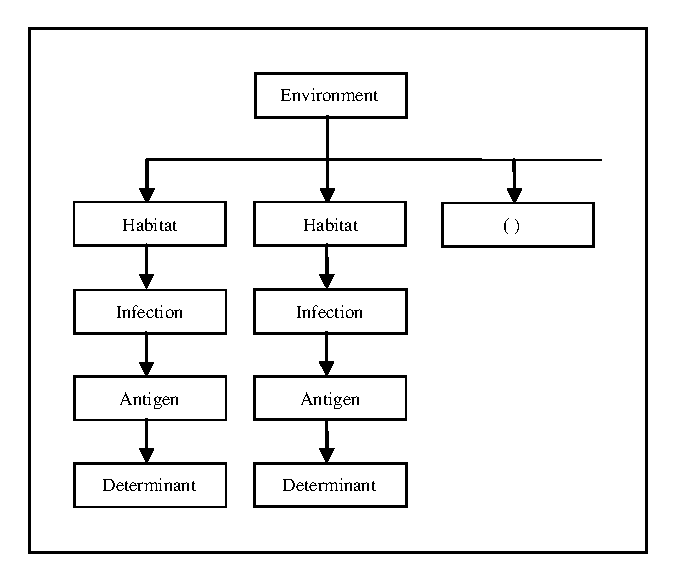
\includegraphics[scale=0.75]{Hosts/hosts-habitats-minimal}
	\caption{Elaboration on figure \ref{fig:tissues:exposures:minimal} to depict the Minimal Habitat Antigenic Exposure Problem (MAHEP)}
	\label{fig:hosts:habitats:minimal}
\end{figure}


%
% Host Exposure Regimes
%
\subsubsection{Host Exposure Regimes}
The HAEP may be specialised with a series of Host Exposure Regimes (HER) in the same manner as the IAEP was specialised with a series of Tissue Exposure Regimes (TER) in Section~\ref{subsec:tissues:paradigm:method:problems}. This reuse is facilitated because both the Tissue and Host paradigms are concerned with strategies for organisation information in the context of unknown scopes and regularities of information exposure. As such, the series of five TER's may be modified for use with the Host Paradigm such that the algorithms remain the same and the parameters are changed from $H$ and $B$ to $P$ and $E$. The following Host specific exposure regimes are defined as AHER, OHER, PHER, RHER, and SHER.

%
% Host Clonal Selection
%
\subsection{Host Clonal Selection}
\label{subsec:hosts:paradigm:realised:algorithms}

%
% Population Host Clonal Selection Algorithm
%
\paragraph{Population Host Clonal Selection Algorithm}
The Tissue Clonal Selection Algorithm (TCSA) defined in Algorithm~\ref{alg:tissues:algorithms:tcsa} describes the general interaction between a Habitat $B$ and a Host $H$. The host paradigm requires a rise in the level of abstraction from a single $H$ to a Population $P$ of $H$ ($P = \{H_1, H_2, H_3, \ldots, H_n\}$) that responds to an Environment $E$ of Habitats $B$. The \emph{Host Clonal Selection Algorithm (HCSA)} defined in Algorithm~\ref{alg:hosts:algorithms:phcsa} describes a general host algorithm that may be specialised based on the concerns and constraints of the Tissue Paradigm, specifically the $HostInteractions$ operation that provides facility for specialising the interactions between hosts. The focus of the HCSA is host interactions within a population, therefore to differentiate the approach from the generational extension (described next), the HCSA may be referred to as a \emph{Population Host Clonal Selection Algorithm (PCSA)} to clarify its relationship with the generational extension.
% minimal
In the tradition of the CCSA and TCSA, one may define a minimal implementation of $HostInteractions$ in which there are no interactions between hosts in the population. This \emph{Minimal Population Host Clonal Selection Algorithm (MP-HCSA)} provides a baseline for comparison with extensions of the PHCSA that facilitates intra-population interactions. 
% single tissue
In addition to no host-interactions, the MP-HCSA codifies the focus of the Host Paradigm on host interactions, taking intra-host concerns considered in the Tissue Paradigm for granted. Specifically, each host in the MP-HCSA has a single tissue ($H = \{T_1\}$), allowing each host to be treated as a generic information processing component in the system.

\begin{algorithm}[htp]
  \SetLine
  \SetKwData{Pop}{P}
	\SetKwData{Env}{E}
  \SetKwFunction{CreateHost}{CreateHost}
  \SetKwFunction{StopCondition}{StopCondition}
  \SetKwFunction{Exposure}{Exposure}
  \SetKwFunction{HostInteractions}{HostInteractions}
  
  \KwIn{\Env, $N_{hosts}$}
	\KwOut{\Pop} 	
	
	\Pop $\leftarrow$0\;
	\For{i$\leftarrow$0 \KwTo $N_{hosts}$}
	{
		$H_i \leftarrow$ \CreateHost{}\;
		\Pop $\leftarrow H_i$\;
	}
	\While{$\neg$\StopCondition{}}
	{
		% do exposure
		\Env.\Exposure{\Pop}\;
		% do interactions	
		\HostInteractions{\Pop}\;
	}
	\Return{\Pop}\;
	\caption{Population Host Clonal Selection.}
	\label{alg:hosts:algorithms:phcsa}
\end{algorithm}

%
% Generational Host Clonal Selection Algorithm (GHCSA)
%
\paragraph{Generational Host Clonal Selection Algorithm}
In addition to a population-based host organisation Section~\ref{sec:hosts:paradigm:architectures} proposed a generational-based host organisation as an extension to the population-based approach in which a new population of hosts is periodically created from an existing population. Algorithm~\ref{alg:hosts:algorithms:ghcsa} defines the \emph{Generational Host Clonal Selection Algorithm (GHCSA)} as an extension of the PHCSA defined in Algorithm~\ref{alg:hosts:algorithms:phcsa}. The $GenerationalChange$ operation defines the frequency of restarts that may for example be based on a consistent number of epochs (population exposures). The $CreatePopulation$ operation defines the mechanism for creating a new $P$ from an existing $P$ that has interacted with the antigenic environment $E$.
% minimal realisation
A minimal implementation of the $CreatePopulation$ can be defined in which the creation of the new population of hosts is independent of the existing population (no interaction). This \emph{Minimal Generational Host Clonal Selection Algorithm (MG-HCSA)} provides a baseline for comparison with extensions of the GHCSA that promotes intra-generational interactions.

\begin{algorithm}[htp]
  \SetLine
  \SetLine
  \SetKwData{Pop}{P}
	\SetKwData{Env}{E}
  \SetKwFunction{CreateHost}{CreateHost}
  \SetKwFunction{StopCondition}{StopCondition}
  \SetKwFunction{Exposure}{Exposure}
  \SetKwFunction{GenerationalChange}{GenerationalChange}  
  \SetKwFunction{CreatePopulation}{CreatePopulation}  
  \SetKwFunction{HostInteractions}{HostInteractions}  
  
  \KwIn{\Env, $N_{hosts}$}
	\KwOut{\Pop} 	
	
	\Pop $\leftarrow$0\;
	\For{i$\leftarrow$0 \KwTo $N_{hosts}$}
	{
		$H_i \leftarrow$ \CreateHost{}\;
		\Pop $\leftarrow H_i$\;
	}
	\While{$\neg$\StopCondition{}}
	{		
		\While{$\neg$\GenerationalChange{}}
		{
			% do exposure
			\Env.\Exposure{\Pop}\;
			% do interactions	
			\HostInteractions{\Pop}\;
		}
		\If{$\neg$\StopCondition{}}
		{
			\Pop $\leftarrow$ \CreatePopulation{\Pop}\;
		}
	}
	\Return{\Pop}\;
	\caption{Generational Host Clonal Selection.}
	\label{alg:hosts:algorithms:ghcsa}
\end{algorithm}


%
% Empirical Assessment
%
\subsection{Empirical Assessment}
\label{subsec:hosts:paradigm:realised:measures}
This section defines a series of empirical measures derived from the measures used in the Tissue Paradigm (Section~\ref{subsec:tissues:paradigm:method:measures}) that provide instantaneous information regarding a given HCSA on Colour Space specialisations of the Habitat Antigenic Exposure Problem. The measures are classified as \emph{system} that provide general holistic information about the algorithm's information state, and \emph{component} that provide generalised information about the algorithm's component information state. As with the Cellular and Tissues Paradigms, an important consideration with the proposed measures in exploratory experimentation is not their absolute value, but rather their relative change in value with changes to the systems being investigated.


%
% System Measures
%
\subsubsection{System Measures}

%
% Population Error
%
\paragraph{Population Error}
The Host Error (HE) defined in Equation~\ref{eq:tissues:measure:he} provides a generalised measure of the error for a single Host Result Set of tissues $H_{rs}$ against a given Habitat of antigenic infection $B$. This measure may be calculate a $H_{rs}$ for each $H$ in a $P$ to formulate an $P_{rs}$ that may be averaged to define a Population error (PE) (see Equation~\ref{eq:hosts:measure:pe}). PE provides an indication of instantaneous average error for each $H_{rs}$ for a given $P_{rs}$ provided by a HCSA in response to an Host Exposure Regime. PE is in the units of the $E$ problem space, for example Euclidean distance for a colour space specialisation.

\begin{equation}
	PopulationError(E, P_{rs}) = \frac{1}{n} \sum_{i=1}^n HostError(B_i, {H_{rs}}_i)
	\label{eq:hosts:measure:pe}
\end{equation}


%
% Population Diversity
%
\paragraph{Population Diversity}
The Host Diversity (HD) measure defined in Equation~\ref{eq:tissues:measure:hd} provides an instantaneous diversity a TCSA. The same approach used in HD for calculating the diversity between repertoires of cells may be used at the population level if the tissues of each host are compressed to a single repertoire. The measures assumes such a reduction permitting the direct calculating of a Bit Frequency Histogram (defined in Algorithm~\ref{alg:tissues:measures:bfh}) for each $H$, permitting the comparison of Hosts using Bit Frequency Difference (defined in Equation~\ref{eq:tissues:measure:bdf}), and ultimately the calculation of diversity according to Equation~\ref{eq:tissues:measure:hd}. For consistency in the measures used in the host paradigm, this measure is re-branded \emph{Population Diversity (PD)}.


%
% Component Measures
%
\subsubsection{Component Measures}

%
% Average Host Diversity (AHD)
%
\paragraph{Average Host Diversity}
The Average Tissue Diversity (ATD) defined in Equation~\ref{eq:tissues:measure:atd} provides an instantaneous measure of the diversity of the average $T$ of a host measured in bits. This measure may be averaged across all hosts in the population $P$ to provide a measure of the average host diversity as the average of the diversity of tissues (defined in Equation~\ref{eq:hosts:measure:ahd}). Alternatively, Average Host Diversity may be calculated as the Host Diversity (defined in Equation~\ref{eq:tissues:measure:hd}) averaged for all hosts in the population. This measure will provide more fidelity for population configuration in which hosts have more than a single tissue. 

\begin{equation}
	AverageHostDiversity(P) = \frac{1}{n}\sum_{i=1}^n AverageTissueDiversity(H_i)
	\label{eq:hosts:measure:ahd}
\end{equation}

%
% Average Host Error (AHE)
%
\paragraph{Average Host Error}
In the same manner as the Average Tissue Error (ATE) in Equation~\ref{eq:tissues:measure:ate}, an average error may be defined that exploits the system-level error calculation for each component of the system. Equation~\ref{eq:hosts:measure:ahe} defines the \emph{Average Host Error (AHE)} that calculates the Population Error (defined in Equation~\ref{eq:hosts:measure:pe}) for $E$ against each host $H$ in $P$, that is averaged by the number of hosts in the population.

\begin{equation}
	AverageHostError(E, P) =  
	% averaged for all H
	\frac{1}{H_n} \sum_{i=1}^{H_n}
	% average error for H_i on E
	\left(\frac{1}{E_n} \sum_{j=1}^{E_n} HostError(B_j, ){H_{rs}}_i)\right)
	\label{eq:hosts:measure:ahe}
\end{equation}


%
% Trends and Behaviours
%
\subsection{Trends and Behaviours}
\label{subsec:hosts:paradigm:realised:behaviours}
This section considers the expected emergent effects and behavioural trends of host-based systems in population and generational architectures as defined in the specific realisations. Although specific to the Host Paradigm, the general behavioural trends are expected to be qualitatively similar to those expected and observed in the Tissue Paradigm. The primarily reason for this is the reuse of varied exposure regimes as a decoupling mechanism between systems and environment for the spatial-temporal regularity or lack there of in the interaction between the two.

%
% Algorithm Mechanism and Strategy
%
\subsubsection{Algorithm Mechanism and Strategy}
Section~\ref{sec:hosts:paradigm:architectures} proposed a population and a generational host architectures providing two different foundational organisations of hosts. This section considers the emergent effects of these two organisations contrasting their mechanism and information management strategies. Table~\ref{tab:hosts:realisation:models:behaviours} provides summary of the two models in these terms.

\begin{table}[ht]
	\centering\small
		\begin{tabular}{lll}
		\toprule
		\textbf{Model} & \textbf{Mechanism} & \textbf{Strategy}  \\ 
		\toprule	
		\emph{Population} & Population of whole systems. & Independent perspectives of problem.\\
		\emph{Generation} & Systems with life-cycles. & Independent perspectives with multiple trials.\\		
		\bottomrule	
		\end{tabular}
	\caption{Summary of the difference in mechanism and strategy between the complementary concerns of host algorithms under discrete exposures.}
	\label{tab:hosts:realisation:models:behaviours}
\end{table}

% population
From a population perspective, each host provides a different independent perspective of the antigenic environment. Inter-host interaction promotes sharing and improvement of the independent toward improving the competence of individuals and ultimately the entire population. This provides a motivation for information management strategies for the population model, highlighting the concerns of information dissemination and localisation in a population (similar to that in the Tissue Paradigm), toward population capability robustness.
% generation
From a generational perspective, the population turnover provides an opportunity for individual perspectives to be refreshed, and for individual host configurations (starting conditions) to be re-trialled in the same or similar antigenic environment. From the abstract perspective, the generational model builds upon the population model, taking the concerns of inter-population interaction for granted, focusing on the mechanism and effects of inter-generational host interactions. The population in each generation is independent from the generation before and after it, thus the motivating concerns of information dissemination and sharing from the population model are directly applicable for motivating intra-generational information management strategies.
% overview
Therefore the general motivations and expectations of the minimal and extended strategies for both host architectures may be summarised as follows:

\begin{enumerate}
	% population
	\item \emph{Population Strategies}
	\begin{enumerate}
		\item Minimal population promotes multiple and potentially variable perspectives on a problem.
		\item Intra-population interaction promotes dissemination between isolated perspectives.
	\end{enumerate}	
	% generation
	\item \emph{Generation Strategies}
	\begin{enumerate}
		\item Minimal generational promotes multiple trials from multiple and potentially variable perspectives on a problem.
		\item Intra-generational interaction promotes dissemination about acquired information between trials.
	\end{enumerate}	
\end{enumerate}

%
% Host Exposure Trends
%
\subsubsection{Host Exposure Trends}
% host disposability
In the tissue paradigm the urgency of acquisition and effective application were promoted by the metaphor of injury by unattended infection, such urgency is not promoted in the host paradigm. Instead, hosts unlike tissues are more expendable as long as some of the hosts population acquire and employ an effective immunity, the `system' (population) will survive. This \emph{disposability of components} is fostered more so in the generational architecture as the mechanism for population assessment and turnover (new component creation) are explicitly defined. 
% independence of perspective
An important consideration in the Host Paradigm is the independence of perspective, in particular the capability of different hosts to respond in varied ways to the same stimulus. This may be investigated by varying host configuration and starting conditions within a population and exposing them to a symmetric antigenic environment to assess emergent effects. 
% why use HER's
Alternatively, the host exposure regimes provide an opportunity for investigating the same effects using the opposite case of the same host configuration exposed to regimes varying in regularity and scope of population exposure. The integration of these two complementary cases represents the pinnacle host-model complexity, where the variation of perspective promoted by the variability of exposure regime provides an idealised and controlled model with strong similarity to model used in the tissue paradigm.
% same effects 
This reuse of exposure regimes in Tissue and Host Paradigms promote similar expectations as to their general effects in terms of \emph{localisation} and \emph{dissemination} across the components of the system although under different constraints. Specifically, a population of host systems interact in different ways from that of the fixed intra-tissue interaction.

% classification
Table~\ref{tab:hosts:her:attributes} classifies the five Host Exposure Regimes in terms of their general attributes, including information \emph{distribution}, \emph{nature}, and \emph{consistency}. One may consider the \emph{distribution} of the exposure of distinct information to the components of the system with the different host exposure regimes. Symmetrical exposure suggests that each component has the opportunity of being exposed to any piece of information in the environment, whereas asymmetrical constraints this expectation. The opportunity may be deterministic, such as a certainty of being exposed to all or some of the information environment or probabilistic in those regimes with a stochastic element. \emph{Scope} provides a general notion as to how much of the system has the opportunity for interacting with the antigenic environment irrespective of the specific information it may be exposed to. The \emph{nature} of the regime defines the basis of the exposure mechanism which directly relates to the consistency of the component-information match ups each each exposure event.

\begin{table}[ht]
	\centering\small
		\begin{tabular}{lllll}
		\toprule
		\textbf{Regime} & \textbf{Distribution} & \textbf{Scope} & \textbf{Nature} & \textbf{Consistency} \\ 
		\toprule
		\emph{AHER} & Symmetrical & System-Wide & Deterministic & Regular \\ 
		\emph{OHER} & Symmetrical & System-Wide & Probabilistic & Semi-Regular \\ 
		\emph{PHER} & Symmetrical & Constrained & Deterministic & Regular \\ 
		\emph{RHER} & Asymmetrical & System-Wide & Probabilistic & Irregular \\ 
		\emph{SHER} & Asymmetrical & System-Wide & Deterministic & Regular \\ 
		\bottomrule
		\end{tabular}
	\caption{Classification of Host Exposure Regimes in terms of general attributes.}
	\label{tab:hosts:her:attributes}
\end{table}


%
% Localisation and Dissemination Trends
%
\subsubsection{Localisation and Dissemination Trends}
Information dissemination promotes \emph{generalised} capability whereas information localisation promotes \emph{specialised} capability. In the tissue paradigm these two contrasting management types were described with regard to their emergent effects in the context of a tissue model, specifically: the `consistency of response' and `spatial organisation of information' respectively. These two effects may be rephrased in the context of the host models as the following:

\begin{enumerate}
	\item \emph{Dissemination}: Consistency in host perspective of the environment across the population and generations.
	\item \emph{Localisation}: Specialisation in host perspective of the environment across the population and generations.
\end{enumerate}

% system-level expectations
The general observational trends for both management types are expected to hold for hosts as they did for investigations into Tissue Paradigm. Specifically, an increase in the population generalisation results in Average Host Error that approaches the Population Error with decrease in system diversity as components are more similar, contrasted with a relative decreased in system error with population specialisation resulting in an increase in system diversity as component become more heterogeneous. 

%
% Paradigm Agenda
%
\subsection{Paradigm Agenda}
\label{subsec:hosts:paradigm:realised:agenda}
The research agenda for this chapter and perhaps the Host Clonal Selection Paradigm is to investigate the population generational models in the context of the expected emergent effects and behavioural trends. Specifically the relative qualitative comparison of the localisation and dissemination of information of different decentralised information management strategies under a variety of information exposure regimes. This may be summarised as follows:

\begin{enumerate}
	\item Investigate strategies to promote intra-population (population model) localisation and dissemination of acquired information.
	\item Investigate strategies to promote intra-generational (generational model) localisation and dissemination of acquired information.
\end{enumerate}


%
% Elicited Immunity
%
\section{Population Elicited Immunity}
\label{sec:hosts:population:elicited}

%
% Antigen Transmission
% 
\subsection{Antigen Transmission}
\label{sec:hosts:population:elicited:theory}
% metaphor
Eliciting an immune response is the way in which the immune system acquires information about the antigenic environment. As reviewed in Section~\ref{sec:hosts:biology:immunisation} this active form of immunisation may occur naturally through normal interactions with pathogen and artificially by exposing a system to harmless molecules with similar features to the antigen of interest that elicits the same response. The artificial elicitation of immunity is the principle behind vaccination's against disease. 
% strategy
In both the artificial and natural cases, eliciting an immune response provides control over what information a host should acquire and when it should be acquired, although this control may or may not reside with the host. 
% abstraction
This control may be abstracted to the general \emph{sampling} of antigen from the environment by a host and future \emph{transmission} to other hosts in the population. This sampling and transmission provides a mechanism by which a given immune system may share information about the antigenic environment with other immune systems in the population. Individual immune systems must collect and store samples of antigen to which they are exposed for transmission to other systems in the population. This mechanism is referred to as the \emph{Antigen Sampling Scheme}. The sampled antigen must then be passed on to other immune systems with which a given immune system interacts. This passing on is referred to as the \emph{Antigen Transmission Scheme}. The antigen sampling mechanism is dependent on the antigenic environment, more explicitly the host antigenic exposure regime the system is subjected to by the environment and other hosts (Antigenic Habitat). The antigen transmission mechanism is dependent on the intra-population (inter-host) interactions facilitated by the population structure, host environment, and any interaction intentions of the individual systems themselves. 

% algorithm
The specialisation of the Population Host Clonal Selection Algorithm (defined in Algorithm~\ref{alg:hosts:algorithms:phcsa}) with an antigen sampling and antigen transmission scheme is called the \emph{Transmission Host Clonal Selection Algorithm (THCSA)}. Algorithm~\ref{alg:hosts:algorithms:thcsa:sample} defines a generic antigen sampling scheme where all habitats exposed to a population are recorded by the hosts for future transmission. The principle of the algorithm is for hosts in a population to inform other hosts in the population in either a controlled or uncontrolled manner regarding antigen of interest, and to allow those hosts to elicit their own internal response. The algorithm is reasonably general, such that it may be specialised in a number of different ways inspired by population-immune system interactions. Two specialisation of the THCSA are defined: (1) uncontrolled transmission scheme inspired by pathogen dynamics, and (2) a host controlled transmission scheme inspired by vaccination dynamics.

\begin{algorithm}[htp]
  \SetLine  
  \SetKwData{Env}{E}
  \SetKwData{Pop}{P}
  \SetKwFunction{SelectHostsToExpose}{SelectHostsToExpose}
  \SetKwFunction{Exposure}{Exposure}
  
  \KwIn{\Env, \Pop}		  
	
	\ForEach{$B_i \in$ \Env}
	{
		$P\prime \leftarrow$ \SelectHostsToExpose{\Pop}\;
		\ForEach{$H_{i}\prime \in P\prime$}
		{
			% exposure
			\Exposure{$H_{i}\prime$, $B_i$}\;
			% store exposures for the host
			$H_{i}\prime$.exposures $\leftarrow B_i$\;
		}		
	}
	\caption{Stored Exposures for Transmission Host Clonal Selection.}
	\label{alg:hosts:algorithms:thcsa:sample}
\end{algorithm}


%
% Pathogen Transmission Dynamics
%
\subsubsection{Pathogen Transmission Dynamics}
A first simple specialisation of the THCSA is to that of an infectious pathogen that may be transmitted from host-to-host. Transmission is achieved via host contact, the number of hosts, and the time of infectiousness (storage time for transmission), all of which are a function of the pathogen. The approach facilitates pathogen behaviour not considered at either the cellular or tissue scales. So-called `host-mediated' pathogenic exposure regimes facilitate emergent information processing that reformulate a given Host Exposure Regimes such as \emph{epidemics} (rapidly spreading), and \emph{pandemics} (complete or close to complete population exposure). The specialisation of the THCSA is defined as follows:

\begin{itemize}
	\item \emph{Sampling Scheme}: Samples are collected when a host is exposed to pathogen from the environment or another host. The longevity of the sample in storage is a property of the infectiousness of the pathogen. A host may be a carrier for more than one pathogen at a given time.
	\item \emph{Transmission Scheme}: A host may transmit a carried pathogen to any systems to which it comes into contact with (for as long as the host is a carrier). Interactions with other immune systems may be random or mediated by proximity, such as in a spatial organisation.
\end{itemize}

% algorithm
The pathogen dynamics inspired approach to the transmission algorithm is called the \emph{Pathogen Transmission Host Clonal Selection Algorithm (PT-HCSA)}. The concerns of pathogen infectiousness and host-carriers are simplified to the collection of all exposed antigenic information (as per Algorithm~\ref{alg:hosts:algorithms:thcsa:sample}), the random selection and transmission of sampled antigen, and the clearing of sampled antigen for each population exposure (algorithm epoch). Two variations of the PT-HCSA are proposed: (1) in which transmissions occur between random pairings of infected hosts, and (2) where transmissions occur between random neighbouring hosts in a one-dimensional fixed-spatial environment. 
% pairing
Algorithm~\ref{alg:hosts:algorithms:pthcsa:randompairings} defines a specialisation of the $HostInteractions$  for random pairing based transmission. 

\begin{algorithm}[ht]
  \SetLine  
  \SetKwData{Pop}{P}
  \SetKwFunction{Exposure}{Exposure}
  \SetKwFunction{SelectRandomHost}{SelectRandomHost}
  \SetKwFunction{SelectRandomExposure}{SelectRandomExposure}
  
  \KwIn{\Pop}		  
  
	\ForEach{$H_i \in$ \Pop}
	{
		% process all hosts that have been exposed
		\If{$H_{i}$.exposures $\neq$0}
		{
			% select a random pair
			$H\prime \leftarrow 0$\;
			\While{$H\prime \equiv H_{i}$}
			{
				$H\prime \leftarrow$ \SelectRandomHost{\Pop}\;
			}
			% select a random antigen to pass on
			$B\prime \leftarrow$ \SelectRandomExposure{$H_{i}$.exposures}\;
			% transmit
			\Exposure{$H\prime$, $B\prime$}\;
		}		
	}
	\caption{Random Pairings for Pathogen Transmission Host Clonal Selection.}
	\label{alg:hosts:algorithms:pthcsa:randompairings}
\end{algorithm}

% spatial pairing
Algorithm~\ref{alg:hosts:algorithms:pthcsa:randomspatial} defines a specialisation of the $HostInteractions$ for the random spatial pairings approach to pathogen transmission where hosts are arranged into a one-dimensional ring structure that limits the random pairing of hosts. Those hosts with sampled exposures transmit a single exposure to a randomly selected spatial neighbour.

\begin{algorithm}[ht]
  \SetLine  
  \SetKwData{Pop}{P}  
  \SetKwFunction{Exposure}{Exposure}
  \SetKwFunction{RandomDouble}{RandomDouble}
  \SetKwFunction{SelectRandomExposure}{SelectRandomExposure}
  
  \KwIn{\Pop}		  
  
	\ForEach{$H_i \in$ \Pop}
	{
		% process all hosts that have been exposed
		\If{$H_{i}$.exposures $\neq 0$}
		{
			$H\prime \leftarrow$0\;
			% select a random host
			\uIf{\RandomDouble{} $< 0.5$}
			{
				\uIf{$H_{i} \equiv H_{n}$}
				{
					$H\prime \leftarrow H_{1}$\;
				}
				\Else
				{
					$H\prime \leftarrow H_{i+1}$\;
				}				
			}
			\Else
			{
				\uIf{$H_{i} \equiv H_{0}$}
				{
					$H\prime \leftarrow H_{n}$\;
				}
				\Else
				{
					$H\prime \leftarrow H_{i-1}$\;
				}		
			}
			% select a random antigen to pass on
			$B\prime \leftarrow$ \SelectRandomExposure{$H_{i}$.exposures}\;
			% transmit
			\Exposure{$H\prime$, $B\prime$}\;
		}		
	}
	\caption{Spatial Pairings for Pathogen Transmission Host Clonal Selection.}
	\label{alg:hosts:algorithms:pthcsa:randomspatial}
\end{algorithm}

This specialisation of THCSA highlights an important property of the transmission principle. Specifically that the antigenic environment (exposure regime to which a population is exposed) may be augmented by intra-population interactions between hosts. Further, the causal influences to inter-population interactions may also be considered indirect influences of host-transmitted pathogenic exposures, such as a hosts proximity to other hosts, host density, or interaction with other hosts from `high pathogenic exposure' areas of the environment. A feature of host-based exposures is that a given host may be a carrier for one or more pathogens to which an interacting system may be exposed. In effect, a given host may represent a micro-environment of antigenic exposures, each potentially providing an exposure regime in and of themselves.


%
% {Vaccination Transmission Dynamics
%
\subsubsection{Vaccination Transmission Dynamics}
The pathogenic dynamics configuration provides a specialisation of the transmission algorithm, in which the sampling scheme is defined by the pathogen, and is thus outside the control of the host system. In this configuration, the host is provided with control over both the sampling and transmission mechanism. A host may select both the antigen to collect and store, and a small sample of host systems from the population to which to transmit the antigen (exposure). This specialisation of the algorithm is inspired by vaccination and inoculation principle from immunology in which a small sample of pathogen is given to a healthy system to illicit immunity to the pathogen. The scheme is simpler than that of the pathogen dynamics scheme in that (1) the host has control over selecting which pathogen to transmit, and (2) the host has control over selecting a `healthy' system to which to transmit a sampled pathogen. The operations for the vaccination specialisation of the THCSA are defined as follows:

\begin{itemize}
	\item \emph{Sampling Scheme}: Samples are collected when a host is exposed to pathogen, although the host has discriminatory control over which pathogen are collected and stored and which are not. Further, the host may decide to discard stored pathogen in the acquisition of additional information from the environment (such as exposure frequency). 
	\item \emph{Transmission Scheme}: A host interacts with systems according to the properties of the environment and the population structure, although the host has control over selection of which encountered system to transmit a sample pathogen to. An example is that a host may select to infrequently inoculate those systems that have a lower probability of being exposed to a given pathogen.
\end{itemize}

As with PT-HCSA, a simplified exposure sampling scheme is used where a randomly selected sampled exposure is transmitted, where sampling is refreshed each epoch. This \emph{Vaccination Transmission Host Clonal Selection Algorithm (VT-HCSA)} (defined in Algorithm~\ref{alg:hosts:algorithms:vthcsa:subset}) has a parameter $N_{vaccinate}$ that defines the number of hosts in the population a single randomly selected host may vaccinate with a single sampled exposure.

\begin{algorithm}[htp]
  \SetLine  
  \SetKwData{Pop}{P}  
  \SetKwFunction{SelectAllExposedHosts}{SelectAllExposedHosts}  
  \SetKwFunction{SelectRandomHosts}{SelectRandomHosts}  
  \SetKwFunction{SelectRandomExposure}{SelectRandomExposure}  
  \SetKwFunction{Exposure}{Exposure}
  
  \KwIn{\Pop, $N_{vaccinate}$}		    
    
	\ForEach{$H_i \in$ \Pop}
	{
		% select random host to vaccinate with
		$P\prime \leftarrow$ \SelectAllExposedHosts{\Pop}\;
		$H\prime \leftarrow$ \SelectRandomHosts{1, $P\prime$}\;
		% select random antigen
		$B\prime \leftarrow$ \SelectRandomExposure{$H\prime$.exposures}\;
		% select a random subset
		$P_{subset} \leftarrow$ \SelectRandomHosts{$N_{vaccinate}$, \Pop}\;
		% expose
		\ForEach{$H_i \in P_{subset}$}
		{
			\Exposure{$H_i$, $B\prime$}\;
		}
	}
	\caption{HostInteractions for Vaccination Host Clonal Selection.}
	\label{alg:hosts:algorithms:vthcsa:subset}
\end{algorithm}

The host selection mechanism provides a powerful tool for the population of immune systems to artificially manipulate the pathogenic exposure regime. This manipulation will likely have the intention of improving `coverage' by the population for the inoculated pathogen. A host may decide to push the limits of the transmission scheme (mass vaccinations) either under special circumstances (adaptive transmission), or all the time. Vaccination of a large sample of the population may provide benefits to the entire population given a `herd immunity' effect. 

%
% Empirical Study
%
\subsection{Transmission Empirical Study}
\label{sec:hosts:population:elicited:study}
%
% Aim
%
\subsubsection{Aim}
The aim of this empirical study was to investigate the Transmission Host Clonal Selection Algorithm, specifically the pathogen and vaccination configurations in the context of their information dissemination and localisation capabilities as compared to the Minimal Population Host Clonal Selection Algorithm under a variety of host exposure regimes. Toward this end, the study had the following goals:

\begin{enumerate}
	\item Investigate the relative effects of the two defined host interaction methods for the uncontrolled pathogen transmission scheme. 
	\item Investigate the relative effects of the controlled elicitation of immunity of the vaccination transmission scheme under different vaccination sample sizes.
\end{enumerate}


%
% Method
%
\subsubsection{Method}

%
% Algorithms
%
\paragraph{Algorithms}
The study considered the Minimal Population Host Clonal Selection Algorithm (MP-HCSA) and the Transmission Host Clonal Selection Algorithm (THCSA), with two specialised configurations: the Pathogen Transmission Host Clonal Selection Algorithm (PT-HCSA) and the Vaccination Transmission Host Clonal Selection Algorithm (VT-HCSA).
% MP-HCSA
MP-HCSA is a specialisation of the HCSA defined in Algorithm~\ref{alg:hosts:algorithms:phcsa}, that was configured with $N_{hosts}=10$. Each $H$ was configured with a single tissue ($N_{tissues}=1$) that was an instance of the Replacement Cellular Clonal Selection Algorithm (RCCSA) defined in Algorithm~\ref{alg:cells:realisation:algorithms:rccsa:exposure}, with the configuration $N_{cells}=50$, $N_{selection}=1$, and $N_{clones}=5$.
% THCSA
The method for sampling all exposures in THCSA defined in Algorithm~\ref{alg:hosts:algorithms:thcsa:sample} was used for both specialised transmission regimes. 
% PT-HCSA
Two different pathogen transmission schemes were investigated, the random pairings scheme defined in Algorithm~\ref{alg:hosts:algorithms:pthcsa:randompairings} referred to as (PT-HCSA-RP), and the random spatial parings defined in Algorithm~\ref{alg:hosts:algorithms:pthcsa:randomspatial} referred to as (PT-HCSA-SP).
% VT-HCSA
The vaccination regime defined in Algorithm~\ref{alg:hosts:algorithms:vthcsa:subset} was used with a small vaccinated set (VT-HCSA-S) $N_{vaccinate}=1$ (10\% of the population) and a large vaccinated set (VT-HCSA-L) $N_{vaccinate}=5$ (50\% of the population).

%
% Problems
%
\paragraph{Problems}
% colour space
The colour space specialisation of the Habitat Antigenic Exposure Paradigm (HAEP) defined in Algorithm~\ref{alg:cells:problem:haep} was used called the Habitat Colour Space Problem (HCSP). The minimal variation of HCSP was used with $N_{habitats}=10$, and $N_{determinants} = N_{antigen} = N_{infections} = 1$. Each $B$ was a Colour Space Pattern (CSP) was randomly generated at the beginning of each run.
% exposure regimes
The five different Host Exposure Regimes (HER) defined in Section~\ref{subsec:hosts:paradigm:realised:problems} were used for the HCSP. These included the AHER where the number of $H$ matched the number of $B$ (one-to-one), SHER, RHER, PHER where $H_{point}$ was fixed at tissue 1, and OHER with $duration=15$.

%
% Experiment
%
\paragraph{Experiment}
Each algorithm used the Maximum Epochs Stop Condition (MESC) defined in Equation~\ref{eq:cells:stopcondition:epochs} with $MaxEpochs=1000$. The four host specific measures defined in Section~\ref{subsec:hosts:paradigm:realised:measures} were collected from the state of the system after the triggering of the stop condition. These included the system measure PE and PD, and the host measures AHE and AHD. Each algorithm and problem received a new and different random number seed each run. Algorithm-Problem combinations were repeated 30 times.

%
% Results
%
\subsubsection{Results}
Table~\ref{tab:hosts:thcsa:results} in Appendix \ref{appendix:results:hosts:transmission} provides a summary of results for each algorithm-problem combination including the mean ($\bar{x}$) and standard deviation ($\sigma$) of collected measure values. Box-and-whisker plots are provided in which the results for each algorithm are aggregated across all HER for a each measure. Figure~\ref{fig:hosts:thcsa:pd:boxplot} shows PD, Figure~\ref{fig:hosts:thcsa:pe:boxplot} shows PE, Figure~\ref{fig:hosts:thcsa:ahd:boxplot} shows AHD, and Figure~\ref{fig:hosts:thcsa:ahe:boxplot} shows AHE.
		
\begin{figure}[htp]
	\centering
		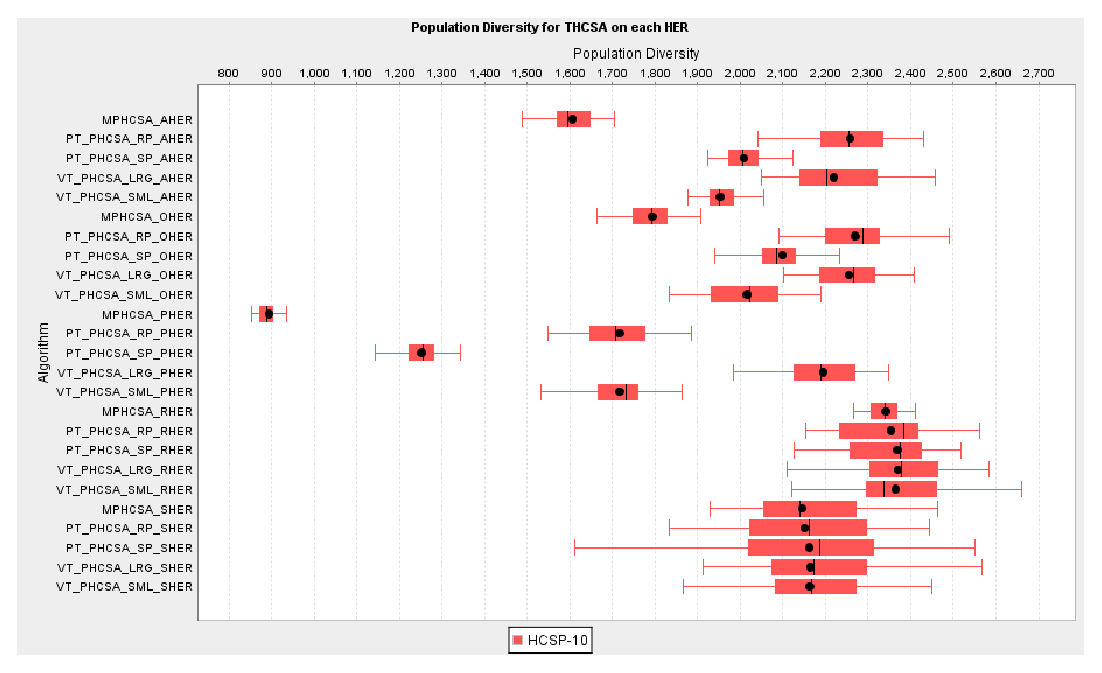
\includegraphics[scale=0.80]{Hosts/THCSA-PD}
	\caption{Box-and-whisker plot of Population Diversity (PD) across all HER for the THCSA study.}
	\label{fig:hosts:thcsa:pd:boxplot}
\end{figure}

\begin{figure}[htp]
	\centering
		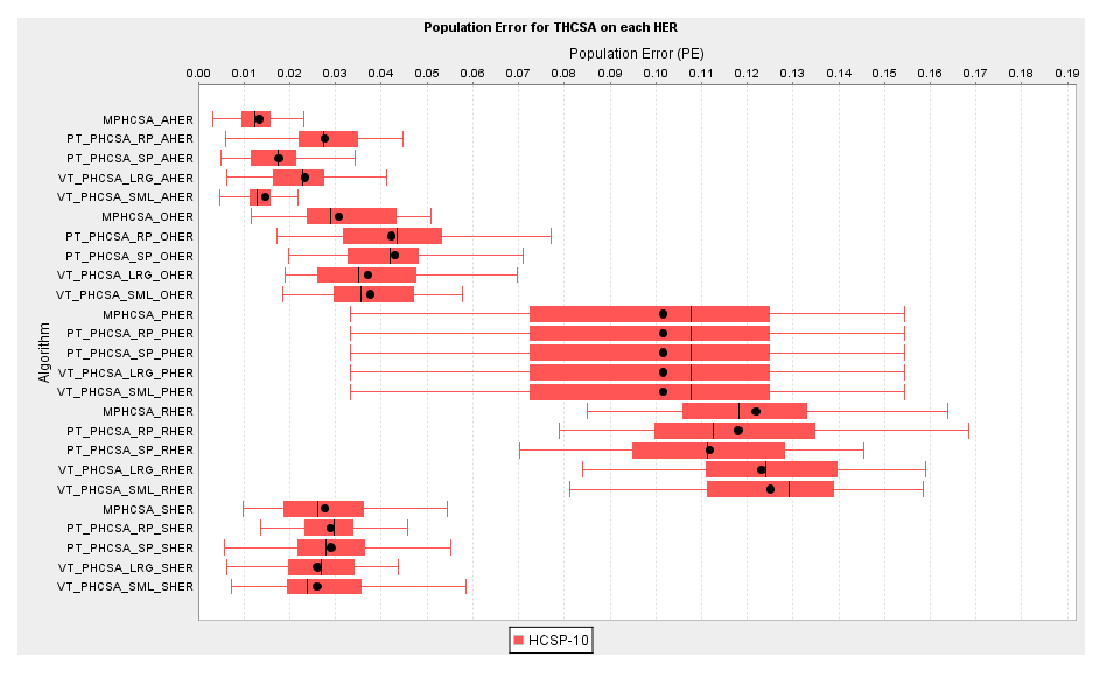
\includegraphics[scale=0.80]{Hosts/THCSA-PE}
	\caption{Box-and-whisker plot of Population Error (PE) across all HER for the THCSA study.}
	\label{fig:hosts:thcsa:pe:boxplot}
\end{figure}

\begin{figure}[htp]
	\centering
		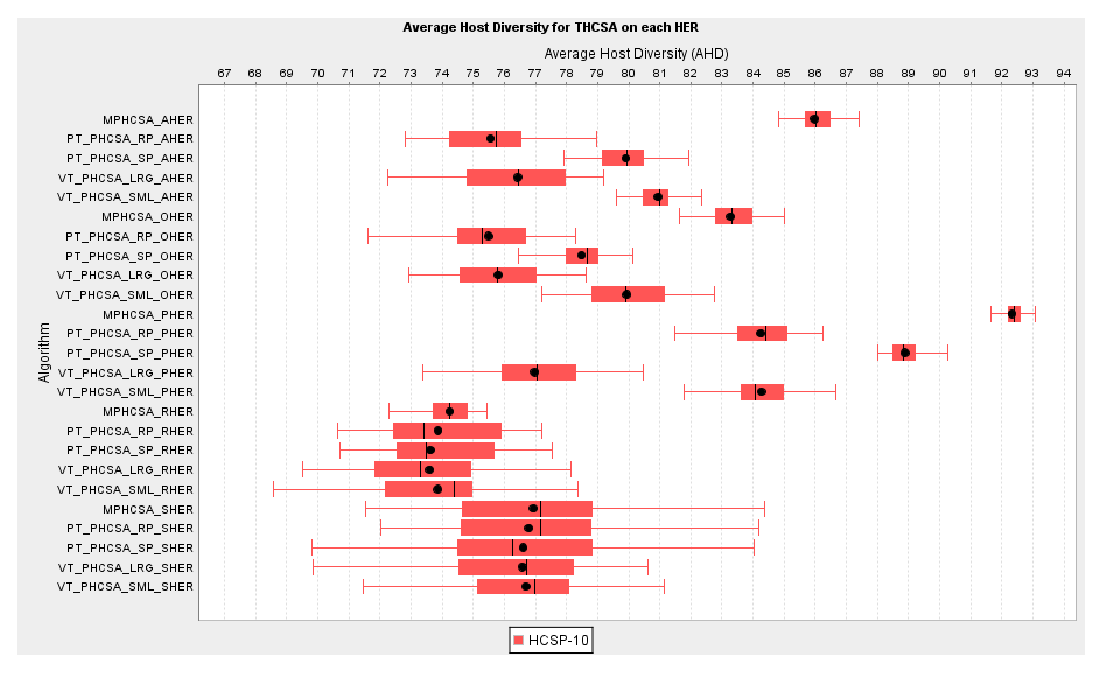
\includegraphics[scale=0.80]{Hosts/THCSA-AHD}
	\caption{Box-and-whisker plot of Average Host Diversity (AHD) across all HER for the THCSA study.}
	\label{fig:hosts:thcsa:ahd:boxplot}
\end{figure}

\begin{figure}[htp]
	\centering
		\includegraphics[scale=0.80]{Hosts/THCSA-AHE}
	\caption{Box-and-whisker plot of Average Host Error (AHE) across all HER for the THCSA study.}
	\label{fig:hosts:thcsa:ahe:boxplot}
\end{figure}

%
% Analysis
%
\subsubsection{Analysis}
This section provides an analysis of the results from the empirical study into the THCSA summarised in Table~\ref{tab:hosts:thcsa:results}. These analyses exploit the trends and expectations outlined in Section~\ref{subsec:hosts:paradigm:realised:behaviours}, and in particular the attributes of host exposure regimes in Table~\ref{tab:hosts:her:attributes}.

%
% Pathogen Dynamics
% (pathogen vs minimal)
%
\paragraph{Pathogen Transmission Trends}
% this section
This section considers the constrained (spatial) and unconstrained random host pairing methods for the pathogen transmission scheme compared to the MP-HCSA that does not facilitate inter-host communication. 
% system
From a system perspective the effect of pathogen transmission was restricted to those exposure regimes with an asymmetric distribution of information to the hosts in the population. Pathogen transmission resulted in an increase in population diversity and population error compared to MP-HCSA on AHER, OHER, and PHER, with no significant difference between the three approaches at the system level on RHER and SHER. The random pairing method resulted in a higher system diversity and system error (increased effect) compared to the constrained spatial random pairing method.
% component
The same trend was observed at the component level with regard to the symmetry in information distribution by the exposure regimes. No significant difference was observed between the three approaches on RHER and SHER with regard to AHD and on SHER with regard to AHE. A relatively large decrease in component diversity and component error was observed with both pathogen transmission schemes on AHER, OHER and PHER. As as was the case with the system measures, the component measures observed an increase in effect with the unconstrained random pairing method than the constrained random spatial pairing method.
% trends
The observations regarding the two pathogen transmission schemes may be generalised to the following trends: 

\begin{enumerate}
	\item Independent perspectives of the information environment are promoted by asymmetrical and not symmetrical information exposure with the chosen host configuration.
	\item Pathogen transmission increases system diversity and error, and decreases component diversity and error on asymmetrical information exposure regimes.
	\item The pathogen dissemination effect was more pronounced with random pairing compared with spatial pairing.
\end{enumerate}

%
% Vaccination Dynamics
% (vaccination vs minimal)
%
\paragraph{Vaccination Size Trends}
% this section
This section considers the vaccination transmission scheme compared to the MP-HCSA, and in particular the effect of varying the number of hosts selected for vaccination per population exposure ($N_{vaccinate}$).
% system
From a system perspective the vaccination scheme demonstrated the same general trend as the pathogen scheme with regard to the restriction of the dissemination effect to those exposure regimes with an asymmetrical information distribution. Vaccination resulted in an increase in system diversity compared to MP-HCSA, and generally no significant change to system error other than a small increase in OHER. The large vaccination size demonstrated a larger increase in system diversity over MP-HCSA than the smaller vaccination size.
% component
From a component perspective vaccination demonstrated a general decrease in the Average Host Diversity and Average Host Error on the asymmetric information distribution exposures. This observed dissemination effect increased with the increase in the vaccination sample size. This result relates to the herd immunity effect, as effective information dissemination is required to facilitate majority coverage in the population under a probabilistic exposure regime. 
% herd immunity in the future
A stronger connection to the herd immunity effect may be investigated in the future by considering a probabilistic variation of PHER with spatial-temporal consistency like the OHER where the dissemination effect for a one or a number of antigenic habitat's could be assessed under a variety of $N_{vaccinate}$ values. The expectation is that the herd immunity effect would be correlated with the improvements to the already measurable dissemination effect (relative decreases in average component diversity and error).
% trends
The observations regarding the vaccination transmission scheme with varied vaccination sizes may be generalised to the following trends: 

\begin{enumerate}
	\item Vaccination promotes dissemination of information that increases system diversity, whilst at the same time decreases average component diversity and error only on exposure regimes with asymmetric information distribution across the population.
	\item The effects of dissemination on the average component is more pronounced with the larger vaccination size (lower relative Average Host Diversity and Error). 
\end{enumerate}

%
% Dissemination Trends
%
\paragraph{Dissemination Trends}
Table~\ref{tab:hosts:thcsa:results:ptvsvt} in Appendix \ref{appendix:results:hosts} contains the results from the random pairing pathogen transmission configuration and the vaccination transmission with large $N_{vacinations}$. These two approaches demonstrated better information dissemination for their respective approaches. This section compares these two different approaches across the five exposure regimes in terms of information dissemination.
% system
From a system perspective there was little significant difference in system diversity and error between the pathogen and vaccination transmission schemes. The only observed significant difference at the system level was on the PHER with an asymmetric information distribution.
% component
The average component perspective provided more insight into the observable differences between the two transmission schemes. The pathogen scheme demonstrated a slightly lower average host diversity on AHER, and a relatively slight increase on the PHER compared the vaccination. The vaccination scheme demonstrated a lower average error on the PHER, whereas the pathogen approach demonstrated a slight decrease in error over vaccination on AHER. This differentiation between the two methods suggests that pathogen transmission provides some benefit on exposure regimes with asymmetric distribution and a system-wide scope, where as vaccination is suited to the constrained scope exposure with asymmetric distribution. This is an intuitive result as one-to-many dissemination is preferred for constrained exposures, and one-to-one dissemination for system-wide exposures. 
% trends
The observations made regarding pathogen and vaccination transmission may be generalised to the following trends:

\begin{enumerate}
	\item There was no significant difference between the pathogen transmission and the vaccination transmission approaches on exposure regimes with symmetric information distribution.
	\item Pathogen transmission schemes provide improved dissemination on system-wide exposure with asymmetric information distribution, whereas the vaccination transmission scheme provides improved dissemination on constrained exposure with asymmetric information distribution.
\end{enumerate}

%
% Conclusions
%
\subsubsection{Conclusions}
This section summarises the findings of the empirical study into the Transmission Host Clonal Selection Algorithm, in terms of the primitives that were the focus of the study and the expectations that motivated the study.

\begin{enumerate}
	\item \emph{Primitives}
		\begin{enumerate}
			\item Pathogen transmission with random pairing provides a viable metaphor for information dissemination via elicitation of response.
			\item Vaccination transmission provides a viable metaphor for information dissemination via elicitation of response that improves with vaccination size.
		\end{enumerate}
	\item \emph{Transmission}
		\begin{enumerate}
			\item There was generally little difference in the dissemination effect between PT-HCSA-RP and VT-HCSA-L, except the pathogen approach demonstrated a relatively slightly better effect on system-wide exposure as opposed the the relatively slightly better effect observed with the vaccination approach on constrained exposure with asymmetrical information distribution.
			\item Exposure regimes with an asymmetric information distribution are required to engender a varied perspective of the antigenic environment in hosts permitting the observation of the dissemination effect.			
		\end{enumerate}				
\end{enumerate}

% confirmation
This last point highlights the important finding from the results that confirmed a base assumption of the empirical investigations into host-based system, which is that the chosen minimal configuration does not result in significantly independent perspectives on the same antigenic environment. This result was demonstrated in the results for the symmetrical RHER and SHER regimes. Alternatively, this result may be interpreted as the confirmation that an exposure regime with an asymmetric information distribution is required to observe varied perspectives of the antigenic environment with the chosen host configuration, allowing the dissemination effect to be observed and measured.
% other things to try
The configuration of transmission schemes were simplistic, providing much room for elaboration and improvement. An important consideration to motivate further investigation is the use of both pathogen and vaccination based transmission schemes in parallel providing the benefits of varied cardinality-based dissemination (one-to-one, one-to-many) suitable for an unknown exposure regime.

%
% Shared Immunity
%
\section{Population Shared Immunity}
\label{sec:hosts:population:shared}

%
% Effector Transmission
%
\subsection{Effector Transmission}
% metaphor
An alternative to actively eliciting an immune response is to allow hosts to sample and share the product of immunisation. 
% strategy
Section~\ref{sec:hosts:biology:immunisation} defined this as passive immunisation highlighting that the immunity provided by inter-host transfer of antibodies is fast, effective, and temporary. This section considers the artificial transplantation of passive immunity between the hosts as a strategy for disseminating specialised acquired information about the antigenic environment between hosts in the population.
% abstraction
The \emph{Shared Immunity} principle is defined as the sharing of acquired immunity between hosts in a population by explicit sampling their own cellular repertoire and transmitting sampled cells to other selected hosts in the population. The sharing requires a sampling scheme of a hosts internal cellular repertoire, and the explicit selection of one or more other sibling host systems in the population to which sampled cells are transmitted. This sampling and transmission facilitates \emph{horizontal sharing} of acquired immunity within the population. The \emph{sampling scheme} is responsible for selecting those mature cells most likely to be useful to those host systems to which the sampled cells are transmitted. There is expected to be a tight coupling between the selection (sampling) of a hosts cellular repertoire and the selection of the recipient host or hosts. Sampled cells will be mature in that they have been produced as a result of an interaction with the antigenic environment. More useful, are those cells that are created from a series of exposures, and thus represent more refined and presently useful information about the environment. The selection of recipient host systems via a \emph{transmission scheme} is the selection of those systems in the population that would most benefit from the sampled acquired immunity. Examples include the transmission of cells from a healthy system (good performance with regard to some system-environment measure), to a system or set of systems that are less healthy (as defined by the same measure). In the absence of such a measure, a good heuristic is the transmission of a representative sample of acquired information to a host that is geographically distant (with regard to the antigenic environment). This heuristic provides a general sharing scheme in which the hosts of the system seek to provide general coverage to the population by sharing acquired immunity. After hosts are selected and the cells are transmitted, the recipient hosts must integrate the received cells into their cellular repertoire. 

\begin{itemize}
	\item \emph{Sampling Scheme}: The identification (selection) and collection of acquired immune cells from a given hosts cellular repertoires for transmission to one or more other hosts (as defined by the hosts cell transmission scheme). Those cells sampled for transmission should be mature with regard to the antigenic environment, and representative of information acquired during the hosts recent exposures. 
	\item \emph{Transmission Scheme}: Requires the selection of sibling hosts within the systems population of immune systems, and the injection (transmission) of sampled cells to selected hosts. The principle concern in the selection of recipient hosts is that the transmitted cells are likely to be useful. This likelihood may be increased by selecting sibling immune systems in the population that are in turn likely to have been subjected to different pathogen and/or at different frequencies (assuming an asymmetric antigenic environment). Once selected, the transmitted cells must be integrated into the recipient systems cellular repertoire.
\end{itemize}

\begin{algorithm}[ht]
  \SetLine
  \SetKwData{Pop}{P}
  \SetKwFunction{RandomHost}{RandomHost}
  \SetKwFunction{RandomTissue}{RandomTissue}
  \SetKwFunction{RandomHost}{RandomHost}
  \SetKwFunction{Remove}{Remove}
  \SetKwFunction{Integrate}{Integrate}
  
  \KwIn{\Pop, $N_{sharers}$, $N_{recipients}$, $N_{sharedcells}$}	
  
	% sharing
	\For{s$\leftarrow$0 \KwTo $N_{sharers}$}
	{
		% select a sharer
		$H_{s} \leftarrow$ \RandomHost{\Pop}\;
		% select cells
		$T\prime \leftarrow$ \RandomTissue{$H_{s}$, $N_{sharedcells}$}\; 
		
		% select recipients
		$P\prime \leftarrow$ \Pop\;
		\While{$P\prime_{n} \neq N_{recipients}$}
		{
			$H\prime \leftarrow$ \RandomHost{$P\prime$}\;
			$P\prime$.\Remove{$H\prime$}\;
		}
		
		% transmit
		\ForEach{$H_{i}\prime \in P\prime$}
		{
			% transmit
			$H_{i}\prime$.\Integrate{$T\prime$}\;
		}
	}  
	\caption{HostInteractions for Shared Immunity Clonal Selection.}
	\label{alg:hosts:algorithms:sihcsa}
\end{algorithm}

% algorithm
The Population Host Clonal Selection Algorithm defined in Algorithm~\ref{alg:hosts:algorithms:phcsa} may be specialised with the the cell sampling and transmission of shared immunity, referred to as the \emph{Shared Immunity Host Clonal Selection Algorithm (SI-HCSA)}. Algorithm~\ref{alg:hosts:algorithms:sihcsa} provides a definition of the $HostInteractions$ operation in which a number of hosts ($N_{sharers}$) select a given number of other hosts in the population ($N_{recipients}$) and share a fixed number ($N_{sharedcells}$) of randomly sampled cells. Transmitted cells are copied from the sharing host and are integrated into the receiving hosts using an integration operation ($Integrate$), and host selection both with regard to sharers and receivers is random ($RandomHost$). This provides a simple realisation of the shared immunity algorithm without cell or host selection bias. 

%
% Empirical Study
%
\subsection{Shared Immunity Empirical Study}
\label{sec:hosts:population:shared:study}

%
% Aim
%
\subsubsection{Aim}
The aim of this empirical study is to investigate the Shared Immunity Host Clonal Selection Algorithm in the context of the information dissemination and localisation capabilities as compared to the Minimal Population Host Clonal Selection Algorithm under a variety of host exposure regimes. Toward this end, the study had the following goals:

\begin{enumerate}
	\item Investigate the relative effects of of small and large sharer and recipient sizes under shared immunity
	\item Investigate the relationships between sharer and recipient sizes and information dissemination.
	\item Assess whether the trend of information dissemination restriction of exposure regimes with asymmetric information dissemination holds.
\end{enumerate}

%
% Method
%
\subsubsection{Method}

%
% Algorithms
%
\paragraph{Algorithms}
The study considered the Minimal Population Host Clonal Selection Algorithm (MP-HCSA) and the Shared Immunity Host Clonal Selection Algorithm (SI-HCSA).
% MP-HCSA
MP-HCSA is a specialisation of the HCSA defined in Algorithm~\ref{alg:hosts:algorithms:phcsa}, that was configured with $N_{hosts}=10$. Each $H$ was configured with a single tissue ($N_{tissues}=1$) that was an instance of the RCCSA defined in Algorithm~\ref{alg:cells:realisation:algorithms:rccsa:exposure}, with the configuration $N_{cells}=50$, $N_{selection}=1$, and $N_{clones}=5$.
% SI-HCSA
SI-HCSA was defined in Algorithm~\ref{alg:hosts:algorithms:sihcsa}, where the integration operation ($Integrate$) was specialised to the Euclidean-based replacement as is used in the RCCSA. The number of shared cells was fixed $N_{sharedcells}=5$ and the number of sharers and recipients were varied. A small number of sharers $N_{sharers}=1$ (10\% of the population) and a large number of sharers $N_{sharers}=5$ (50\% of the population) were assessed with a small number of recipients $N_{recipients}=1$ (10\% of the population) and a large number of recipients $N_{recipients}=5$ (50\% of the population). 

%
% Problems
%
\paragraph{Problems}
The same Habitat Colour Space Problem and Host Exposure Regimes were used as was defined for the THCSA empirical study in Section~\ref{sec:hosts:population:elicited:study}.

%
% Experiment
%
\paragraph{Experiment}
The same experimental setup was used as was defined for the THCSA empirical study in Section~\ref{sec:hosts:population:elicited:study}.

%
% Results
%
\subsubsection{Results}
Table~\ref{tab:hosts:sihcsa:results} in Appendix \ref{appendix:results:hosts:shared} provides a summary of results for each algorithm-problem combination including the mean ($\bar{x}$) and standard deviation ($\sigma$) of collected measure values.  Box-and-whisker plots are provided in which the results for each algorithm are aggregated across all HER for each measure. Figure~\ref{fig:hosts:sihcsa:pd:boxplot} shows PD, Figure~\ref{fig:hosts:sihcsa:pe:boxplot} shows PE, Figure~\ref{fig:hosts:sihcsa:ahd:boxplot} shows AHD, and Figure~\ref{fig:hosts:sihcsa:ahe:boxplot} shows AHE.

\begin{figure}[htp]
	\centering
		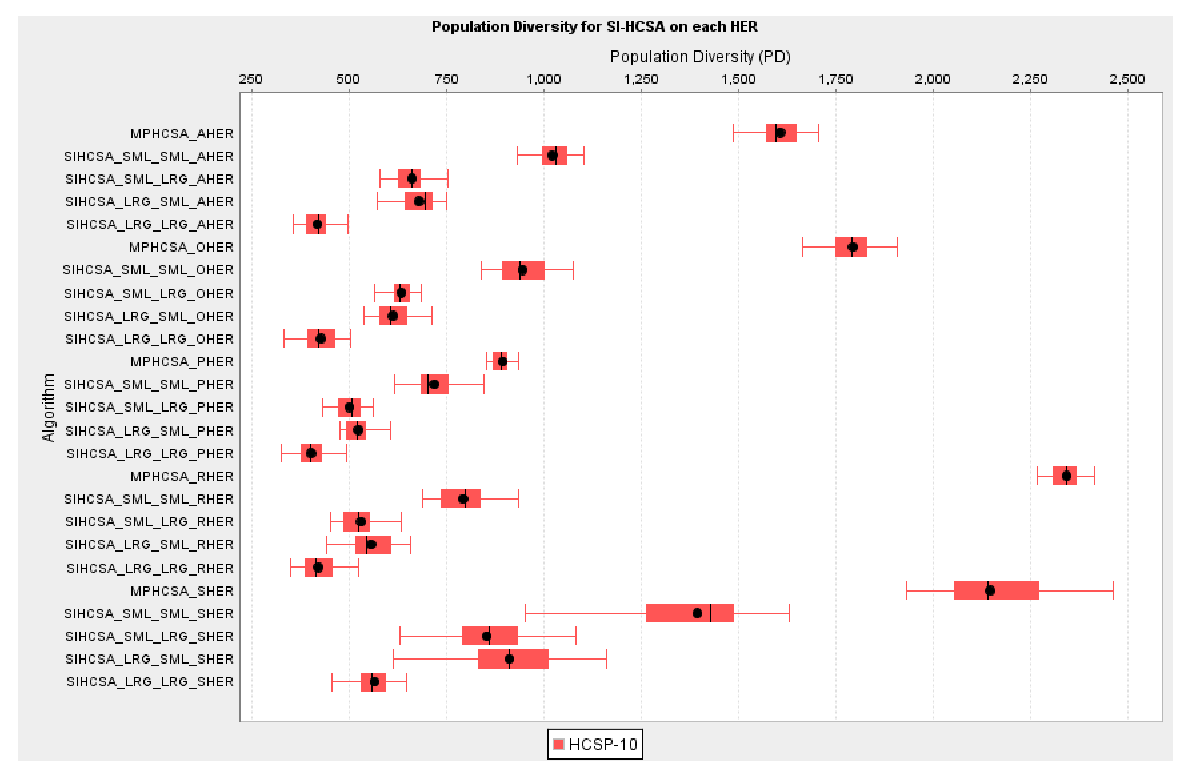
\includegraphics[scale=0.70]{Hosts/SI-HCSA-PD}
	\caption{Box-and-whisker plot of Population Diversity (PD) across all HER for the SI-HCSA study.}
	\label{fig:hosts:sihcsa:pd:boxplot}
\end{figure}

\begin{figure}[htp]
	\centering
		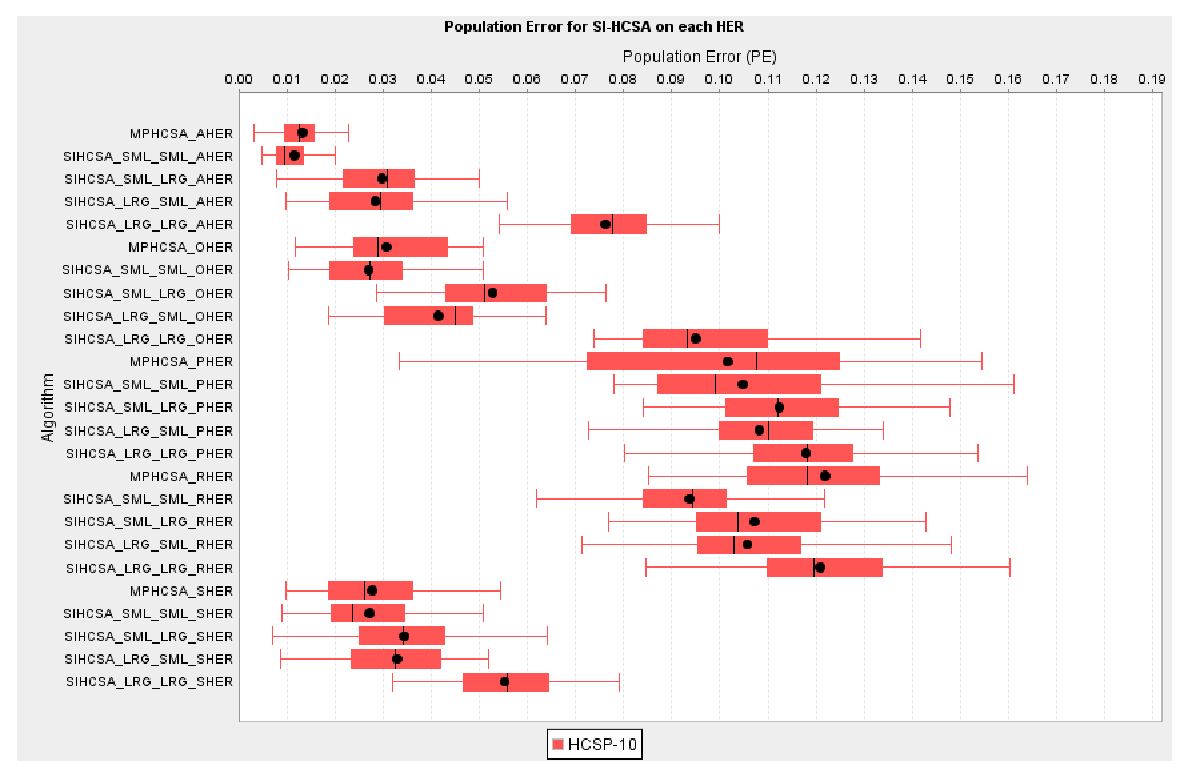
\includegraphics[scale=0.70]{Hosts/SI-HCSA-PE}
	\caption{Box-and-whisker plot of Population Error (PE) across all HER for the SI-HCSA study.}
	\label{fig:hosts:sihcsa:pe:boxplot}
\end{figure}

\begin{figure}[htp]
	\centering
		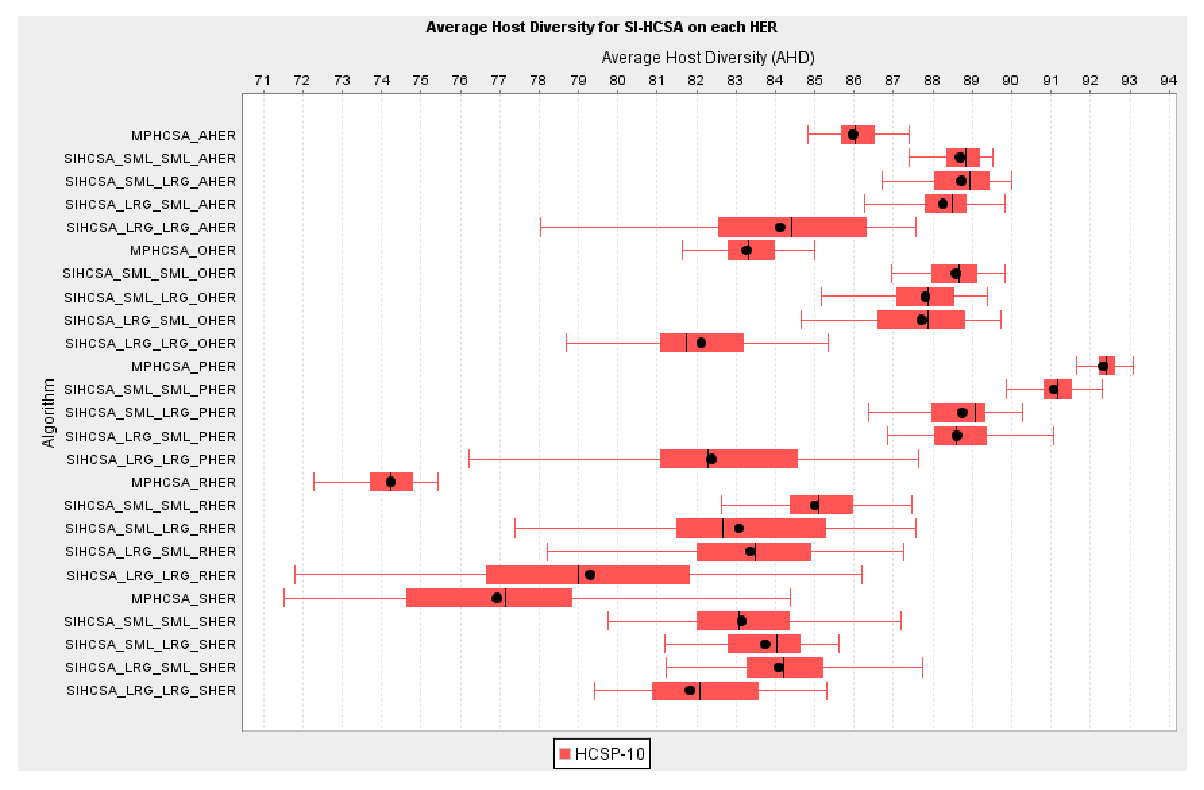
\includegraphics[scale=0.70]{Hosts/SI-HCSA-AHD}
	\caption{Box-and-whisker plot of Average Host Diversity (AHD) across all HER for the SI-HCSA study.}
	\label{fig:hosts:sihcsa:ahd:boxplot}
\end{figure}

\begin{figure}[htp]
	\centering
		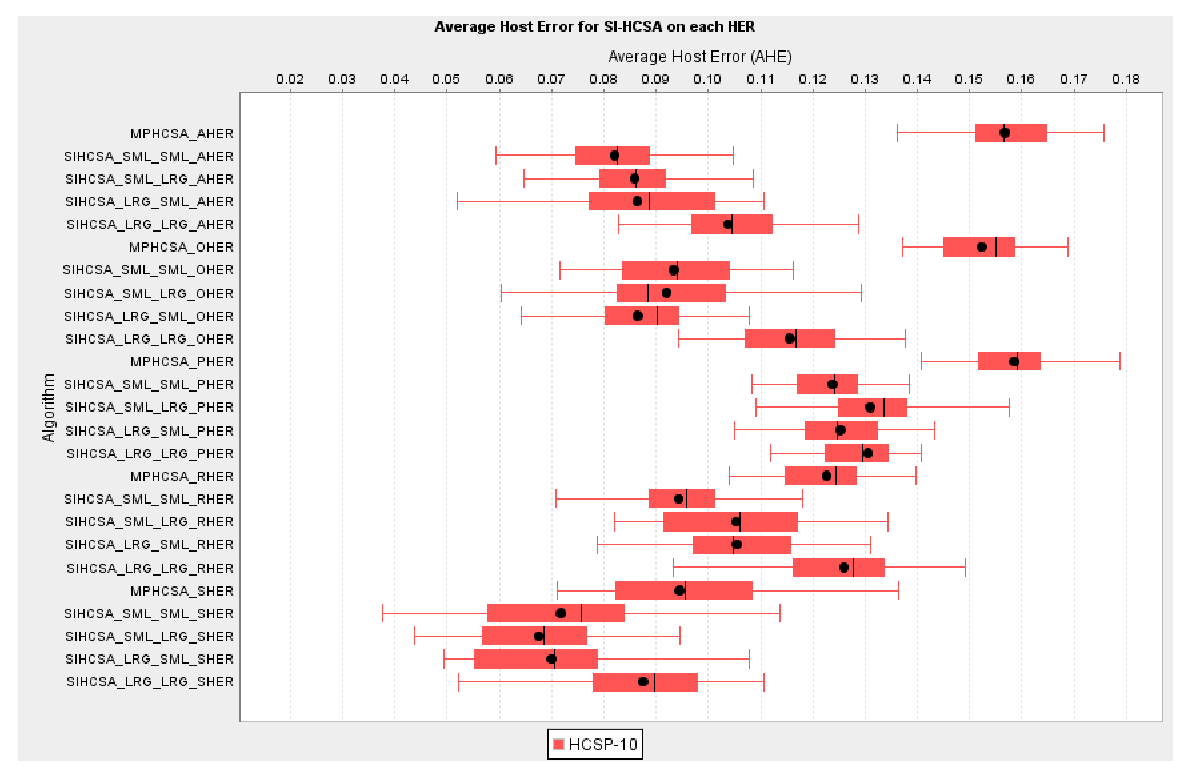
\includegraphics[scale=0.70]{Hosts/SI-HCSA-AHE}
	\caption{Box-and-whisker plot of Average Host Error (AHE) across all HER for the SI-HCSA study.}
	\label{fig:hosts:sihcsa:ahe:boxplot}
\end{figure}


%
% Analysis
%
\subsubsection{Analysis}
This section provides an analysis of the results from the empirical study into the SI-HCSA summarised in Table~\ref{tab:hosts:sihcsa:results}. These analyses exploit the trends and expectations outlined in Section~\ref{subsec:hosts:paradigm:realised:behaviours} regarding information dissemination between the hosts in the population.

%
% Share Size Trends
%
\paragraph{Sharer Size Trends}
This section is concerned with the effect of the number of hosts sharing acquired immunity in the population ($N_{sharers}$), irrespective of the number of recipients ($N_{recipients}$). As such, the observations are taken as the general trends in the small and large number of sharer hosts. 
% system
From a system perspective the Population Diversity was generally lower with sharing compared to MP-HCSA across all exposure regimes. The increase in sharer size generally resulted in a decrease in diversity. A similar relationship was observed with system error, where sharing generally resulted in an increase in system error compared to MP-HCSA, an effect that increased with the number of sharers (increase in share size increased system error). 
% component
From a component perspective shared immunity resulted in a general decrease in the Average Host Diversity than MP-HCSA. This effect decreased with the increase in number of sharing hosts, such that a AHD approached MP-HCSA on the AHER, OHER, and RHER domains. Interestingly, a similar effect was observed with the Average Host Error that was generally lower than MP-HCSA, although increased with the increase in the sharer size. 
% trends
This correlation in relationships at the system and component level with share size demonstrates a disruptive and information dissemination effect at the system and component level respectively that generally results in increased disruption at both scales with the increase in the number of hosts sharing immunity. The observations may be generalised to the following trends: 

\begin{enumerate}
	% system
	\item \emph{System}
		\begin{enumerate}
			\item Shared immunity results in a generally lower population diversity and generally higher population error than MP-HCSA.
			\item Increase in sharing size results in increase in system level effects, specifically decreases in system diversity and increases in system error.
		\end{enumerate}

	% component
	\item \emph{Component}
		\begin{enumerate}
			\item Shared immunity results in a general increase in Average Host Diversity, and a general decrease in Average Host Error compared to MP-HCSA.
			\item Increase in a decrease in component level effects with an increase a decrease in Average Host Diversity, and a general increase in Average Host Error.
		\end{enumerate}
\end{enumerate}


%
% Recipient Size Trends
%
\paragraph{Recipient Size Trends}
This section considers the effects of varying the number of recipient hosts ($N_{recipients}$) irrespective of the number of hosts sharing. As such, the results are generalised across the configuration values for the number of sharers ($N_{sharers}$). 
% system
From a system perspective Population Diversity and Error exhibited the same trends both with regard to the comparison to MP-HCSA and with regard to the increase in the number of recipients increasing the disruptive effect of sharing at the system level.
% component
The same relationship was demonstrated at the component level with a general increase in diversity and decrease in error compared to MP-HCSA, and the increased disruption (decreased average diversity and increased average error) with the increased in the number of recipients.
% trends
These observation demonstrate an important symmetry in general behaviour between the number of hosts sharing acquired immunity and the number of hosts receiving acquired immunity. In particular increasing either results in a increase in the disruption at the system level and disruption to the dissemination of information at the component level. These observations may be summarised in the following generalised trends:

\begin{enumerate}
	\item The system and component-level effects of recipient size mirror the effect trends of number of sharing hosts. 		
	\begin{enumerate}
		\item System diversity decrease and system error which increases with recipient size. 
		\item Component diversity increases and component error decreases, an effect that decreases with recipient size.
	\end{enumerate}
\end{enumerate}

%
% Sharer and Recipient Relationship Trends
%
\paragraph{Sharer and Recipient Relationship Trends}
This section considers the trends in the relationships between the number of hosts sharing and the number of hosts receiving shared immunity, not considerating the comparison the MP-HCSA. 
% system
From a system perspective the highest population diversity was observed with a one-to-one relationship, whereas the lowest population diversity was observed with a many-to-many configuration. Generally there was no significant difference between one-to-many and many-to-one configurations across the exposure regimes, with PHER as the exception. The same general trend was observed with regard to population error, where the lowest error was achieved by one-to-one and the largest system error was achieved by many-to-many. Interestingly, no significant difference in system error was observed between SI-HCSA-SS and MP-HCSA on all exposure regimes except RHER where one-to-one sharing resulted in a lower system error.
% component
The component perspective demonstrated the same general trend where the highest average component diversity and least average component error were observed with the one-to-one configuration, and the most disruption in diversity and error caused by the large scale sharing in the many-to-many configuration. Also consistent was the lack of significant difference in effect between the one-to-many and many-to-one configurations. 
% trends
The consistency of the dissemination effect in the relationship between both the number of sharer and recipient hosts was confirmed both in the extreme cases with the least and most disruption caused by the least and the most amount of sharing, and in the intermediate cases confirming the symmetry in behaviour. These observations may be summarised in the following generalised trends:

\begin{enumerate}
	\item Generally no significant difference in assessed measures between one-to-many or many-to-one with regard to the number of sharers and recipients across all HER.
	\item The least disruptive system effect was observed with one-to-one, whereas the largest disruptive system effect was observed with many-to-many sharing.
	\item The best dissemination effect at the component level was observed with one-to-one sharing, whereas the worst disruptive effect at the component level was observed with many-to-many sharing.
\end{enumerate}


%
% Conclusions
%
\subsubsection{Conclusions}
This section summarises the findings of the empirical study into the Shared Immunity Host Clonal Selection Algorithm, in terms of the primitives that were the focus of the study and the expectations that motivated the study.

\begin{enumerate}
	\item Large scale sharing provides a disruptive effect at the system and component level.
	\item Small scale sharing minimises the disruptive effect at the system level and maximise the dissemination effect at the component level.
\end{enumerate}

An interesting aspect of artificial passive immunity is the concern that such shared information is initially useful although such utility is temporary. This property is expected to vary with exposure regime and provides an important extension to the investigation into the SI-HCSA.

%
% Maternal Immunity
%
\section{Generational Maternal Immunity}
\label{sec:hosts:generational:maternal}

%
% Generational Transmission
%
\subsection{Generational Transmission}
\label{sec:hosts:generational:maternal:theory}
% metaphor
Maternal immunity involves progeny receiving antibodies and immune cells from the mother, both across the placenta and in breast milk (mucosal immunity). This type of immunity is referred to as natural-passive immunity because the conferred acquired immune information is passed between the hosts without eliciting an immune response.
% strategy
Maternal immunity provides a strategy for one generation of immune systems with lifetime acquired immunity to transfer such acquired knowledge to the following generation.
% abstraction
As with intra-population sharing of acquired immunity via passive means in Shared Immunity (Section~\ref{sec:hosts:population:shared}), a cell sampling and transmission scheme are required. The concerns of cell sampling are predominantly similar to the concerns highlighted in the Transmission and Shared Immunity Host Clonal Selection Algorithms. It is important to highlight the trade-off of the sampled cells and their effect on freshly instantiated host systems. A selection of a sample that is too large or contains many dominant (with respect to clonal selection) pieces of acquired information (memory cells) will cause the recipient systems to (in effect) represent continuances of the transmitting host. The sample should be diverse and representative, and likely contain many effector cells. The selection of effector cells for transmission is useful for a number of reasons. Firstly, the biological inspiration (maternal, and more importantly mucosal immunity) confers mostly this type of acquired immunity in the form of antibodies. 

\begin{itemize}
	\item \emph{Sampling Scheme}: The selection of mature acquired immune cells from host systems to be removed and transmitted to host systems of the subsequent generation. The selection scheme should draw a representative sample of the information acquired by the system over the course of its lifetime (trial period).
	\item \emph{Transmission Scheme}: The selection of instantiated host systems of the subsequent generation by hosts of the present generation to which sample acquired immune systems cells will be transmitted. A simple host selection scheme is the selection of progeny host systems.
\end{itemize}


% parent-child
The host transmission scheme requires the selection of hosts in the subsequent generation to receive the sampled cells. A natural implementation of this scheme is the selection of progeny hosts. Specifically, the selection of hosts in the subsequent generation by hosts in the present generation, to which they are responsible for instantiating. The parent-child transmission scheme may result in the formation of independent generational host-lines given the asexual basis of the approach. The concern of this effect is that if a given host system is lost, then the information acquired by that hosts generational line is also lost. This concern may be addressed by relaxing the parent-child transmission constraint, and allowing parent-hosts to potentially transmit to any host in the child generation. A biological basis for this configuration may be the use of manufactured formulae, or the use of a wet-nurse. An example of a decoupled transmission scheme is random host selection, with reselection. The reselection allows a given host in the child generation to potentially receive acquired immune information from more than one parent host system. The transmission of cells to non-child hosts provides redundancy between host lines, if there is a relationship between parent-child that may affect host-loss (such as reproduction in a hazardous spatial environment). A one-to-many transmission scheme between the generations will also foster redundancy of acquired information between the generations. The concern in a host system receiving acquired immune information from more than one host, is that the child system may become overly biased by the previous generation. A parent-child (one-to-one) transmission scheme limits the scope of received acquired immune information to a single host of the previous generation's perspective.

% MG-HCSA
The Minimal Generational Host Clonal Selection Algorithm (MG-HCSA) of the generational algorithm defined in Algorithm~\ref{alg:hosts:algorithms:ghcsa} provides a basis for comparison with a maternal immunity approach as it promotes independent generations. Algorithm~\ref{alg:hosts:algorithms:ghcsa:mghcsa} provides a definition of the $CreatePopulation$ operation for the MG-HCSA. Equation~\ref{eq:hosts:algorithms:generationalchange} provides a generational change trigger based on a number of population exposures or epochs, where a user specified parameter $N_{genepochs}$ defines the maximum number of epochs before a generational change is triggered.

% MG-HCSA
\begin{algorithm}[htp]
  \SetLine
  \SetKwData{Pop}{P}
  \SetKwFunction{CreateHost}{CreateHost}
  
  \KwIn{\Pop, $N_{hosts}$}
	\KwOut{$P\prime$} 	
	
	$P\prime \leftarrow$0\;
	\For{i$\leftarrow$0 \KwTo $N_{hosts}$}
	{
		$H_i \leftarrow$ \CreateHost{}\;
		$P\prime \leftarrow H_i$\;
	}
	\Return{$P\prime$}\;
	\caption{CreatePopulation for the Minimal Generational Clonal Selection.}
	\label{alg:hosts:algorithms:ghcsa:mghcsa}
\end{algorithm}


% stop condition
\begin{equation}
	GenerationalChange(Epoch_i) = \left(Epoch_i \geq N_{genepochs} \right)
	\label{eq:hosts:algorithms:generationalchange}
\end{equation}

% MI-HCSA
A \emph{Maternal Immunity Host Clonal Selection Algorithm (MI-HCSA)} may be defined as the realisation of intra-generational sharing of acquired immunity that may be specialised to parent-child based sharing. Algorithm~\ref{alg:hosts:algorithms:mihcsa} defines the $CreatePopulation$ operation for parent-child based maternal immunity, where the amount of inter-generational sharing is defined by a user defined parameterL $N_{maternalcells}$. 

% parent-child
\begin{algorithm}[htp]
  \SetLine
  \SetKwData{Pop}{P}
  \SetKwFunction{SelectRandomTissue}{SelectRandomTissue}
  \SetKwFunction{CreateHost}{CreateHost}
  \SetKwFunction{Integrate}{Integrate}
  
  \KwIn{\Pop, $N_{maternalcells}$}
	\KwOut{$P\prime$} 
		
	$P\prime \leftarrow$0\;
	\ForEach{$H_i \in$ \Pop}
	{
		% sample from parent
		$T\prime_i \leftarrow$ \SelectRandomTissue{$H_{i}$, $N_{maternalcells}$}\; 
		% create normally
		$H\prime_i \leftarrow$ \CreateHost{}\;
		% integrate
		$H\prime_i$.\Integrate{$T\prime_i$}\;
		% store in new pop
		$P\prime \leftarrow H\prime_i$\;
	}
	\Return{$P\prime$}\;
	\caption{CreatePopulation for Maternal Immunity Clonal Selection.}
	\label{alg:hosts:algorithms:mihcsa}
\end{algorithm}

%
% Empirical Study
%
\subsection{Maternal Immunity Empirical Study}
\label{sec:hosts:generational:maternal:study}
%
% Aim
%
\subsubsection{Aim}
The aim of this empirical study is to investigate the Maternal Immunity Host Clonal Selection Algorithm in the context of the information dissemination and localisation capabilities as compared to the Minimal Generational Host Clonal Selection Algorithm under a variety of host exposure regimes. Toward this end, the study had the following goals:

\begin{enumerate}
	\item Compare and contrast generational clonal selection with and without inter-generational sharing. 
	\item Investigate the dissemination of information effect and its disruption by varying the amount of inter-generational sharing. 
\end{enumerate}

%
% Method
%
\subsubsection{Method}
	
%
% Algorithms
%
\paragraph{Algorithms}
The study considered the Minimal Generational Host Clonal Selection Algorithm (MG-HCSA) and the Maternal Immunity Host Clonal Selection Algorithm (MI-HCSA).
% MG-HCSA
MG-HCSA is a specialisation of the HCSA defined in Algorithm~\ref{alg:hosts:algorithms:ghcsa}, that was configured with $N_{hosts}=10$. Each $H$ was configured with a single tissue ($N_{tissues}=1$) that was an instance of the RCCSA defined in Algorithm~\ref{alg:cells:realisation:algorithms:rccsa:exposure}, with the configuration $N_{cells}=50$, $N_{selection}=1$, and $N_{clones}=5$. The $CreatePopulation$ operation for the MG-HCSA was realised as the creation of a new population of hosts each generational change as defined in Algorithm~\ref{alg:hosts:algorithms:ghcsa:mghcsa}, and the epoch generational change condition defined in Equation~\ref{eq:hosts:algorithms:generationalchange} with $N_{genepochs}=100$.
% MI-HCSA
The MI-HCSA with assessed with the parent-child specialisation of the $CreatePopulation$ operation defined in Algorithm~\ref{alg:hosts:algorithms:mihcsa}. The number of cells selected for inter-generational sharing was assessed with three different values as follows: small $N_{maternalcells}=5$ (10\% of the hosts repertoire), medium $N_{maternalcells}=10$ (20\% of the hosts repertoire), and large $N_{maternalcells}=25$ (50\% of the hosts repertoire).

%
% Problems
%
\paragraph{Problems}
The same Habitat Colour Space Problem and Host Exposure Regimes were used as was defined for the THCSA empirical study in Section~\ref{sec:hosts:population:elicited:study}.

%
% Experiment
%
\paragraph{Experiment}
The same experimental setup was used as was defined for the THCSA empirical study in Section~\ref{sec:hosts:population:elicited:study}, except the maximum number of epochs of the EOSC stop condition was decreased from 1000 to 999. This configuration change was made such that the final measures recorded reflected the state of the system after 10 generations of 100 epochs before the last generational change (at the tenth generation).

%
% Results
%
\subsubsection{Results}
Table~\ref{tab:hosts:mihcsa:results} in Appendix \ref{appendix:results:hosts:maternal} provides a summary of results for each algorithm-problem combination including the mean ($\bar{x}$) and standard deviation ($\sigma$) of collected measure values.  Box-and-whisker plots are provided in which the results for each algorithm are aggregated across all HER for a each measure. Figure~\ref{fig:hosts:mihcsa:pd:boxplot} shows PD, Figure~\ref{fig:hosts:mihcsa:pe:boxplot} shows PE, Figure~\ref{fig:hosts:mihcsa:ahd:boxplot} shows AHD, and Figure~\ref{fig:hosts:mihcsa:ahe:boxplot} shows AHE.

\begin{figure}[htp]
	\centering
		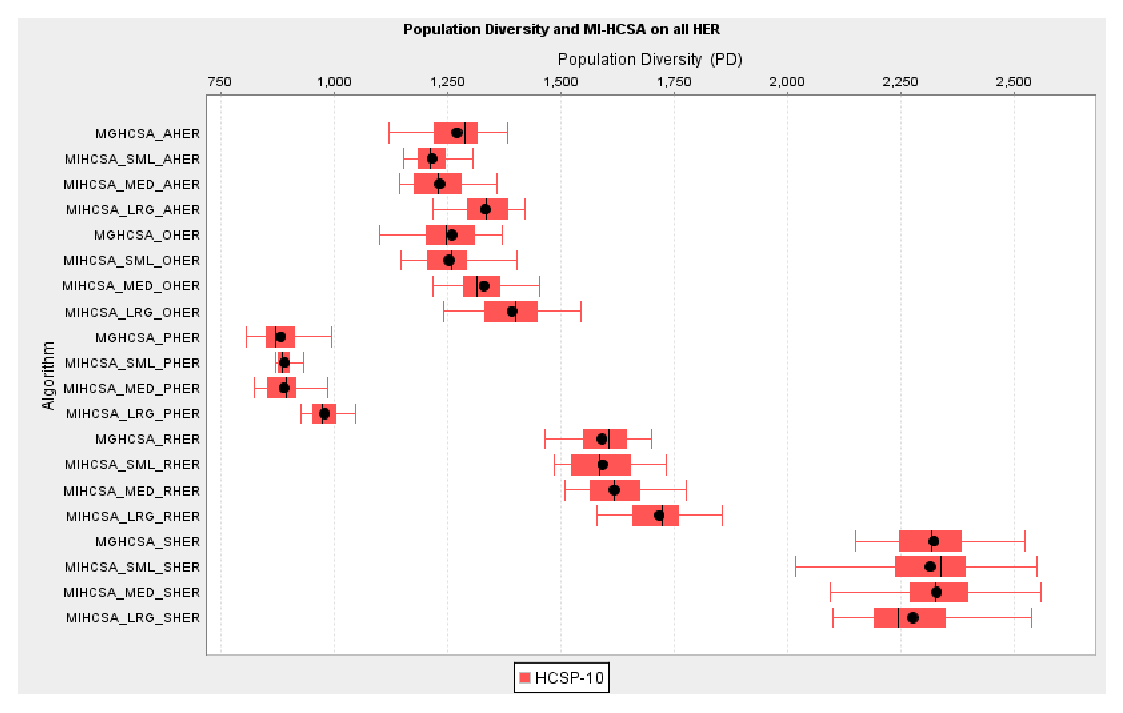
\includegraphics[scale=0.70]{Hosts/MI-HCSA-PD}
	\caption{Box-and-whisker plot of Population Diversity (PD) across all HER for the MI-HCSA study.}
	\label{fig:hosts:mihcsa:pd:boxplot}
\end{figure}

\begin{figure}[htp]
	\centering
		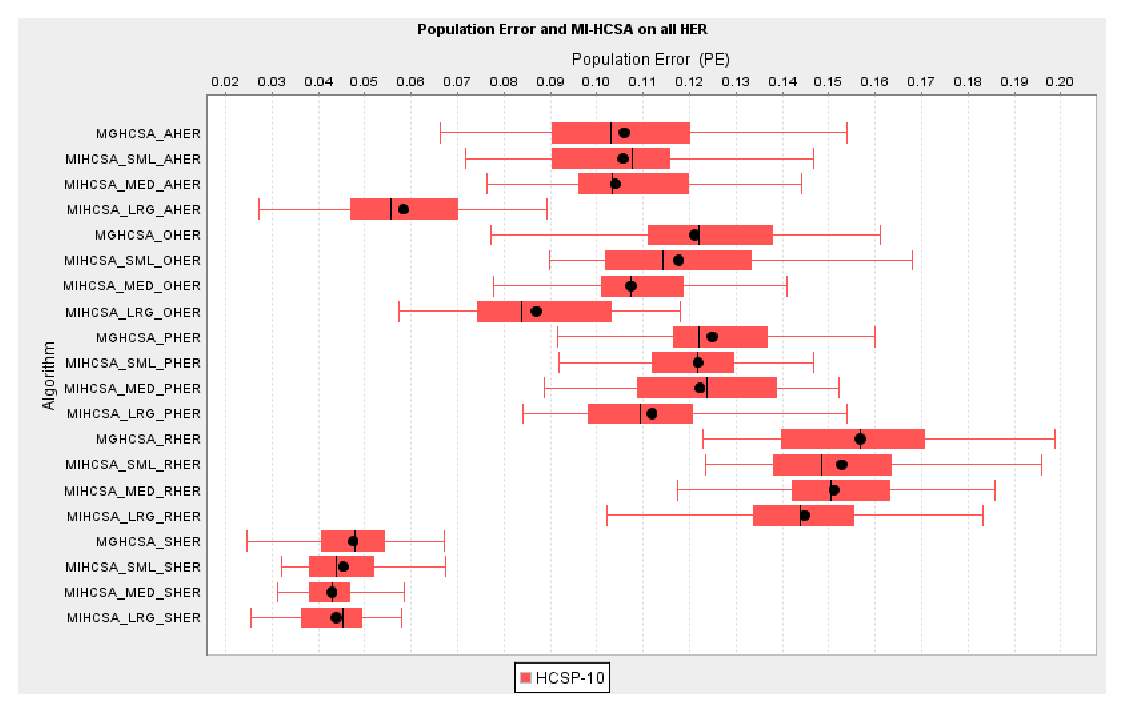
\includegraphics[scale=0.70]{Hosts/MI-HCSA-PE}
	\caption{Box-and-whisker plot of Population Error (PE) across all HER for the MI-HCSA study.}
	\label{fig:hosts:mihcsa:pe:boxplot}
\end{figure}

\begin{figure}[htp]
	\centering
		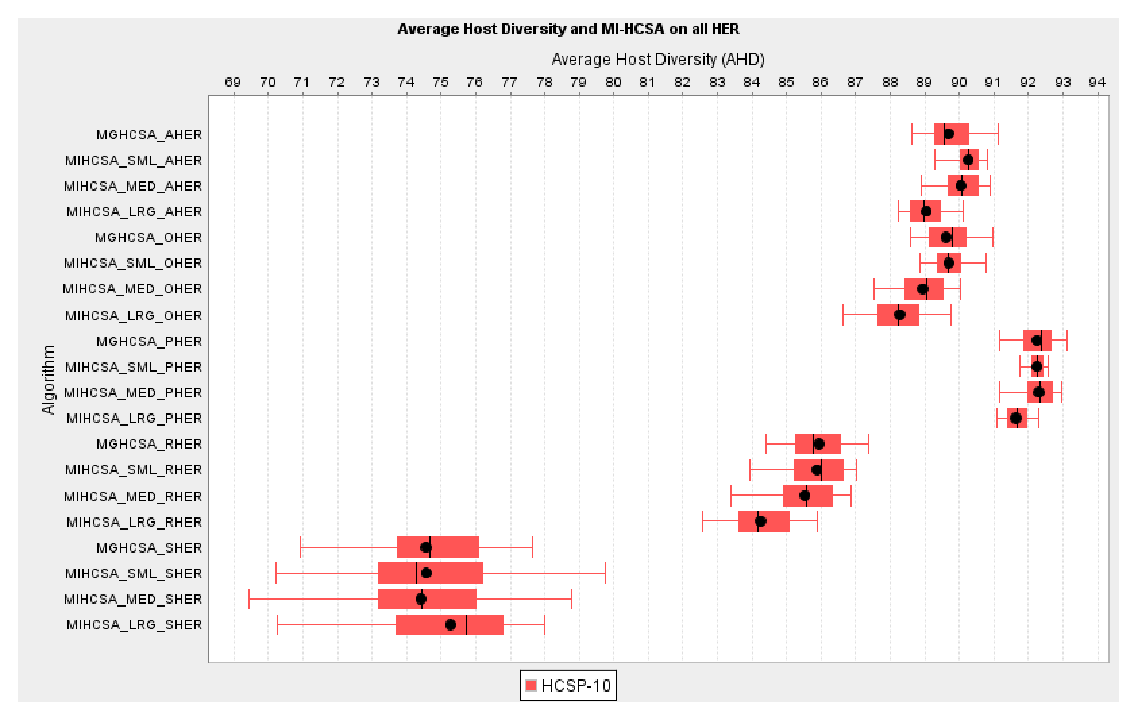
\includegraphics[scale=0.70]{Hosts/MI-HCSA-AHD}
	\caption{Box-and-whisker plot of Average Host Diversity (AHD) across all HER for the MI-HCSA study.}
	\label{fig:hosts:mihcsa:ahd:boxplot}
\end{figure}

\begin{figure}[htp]
	\centering
		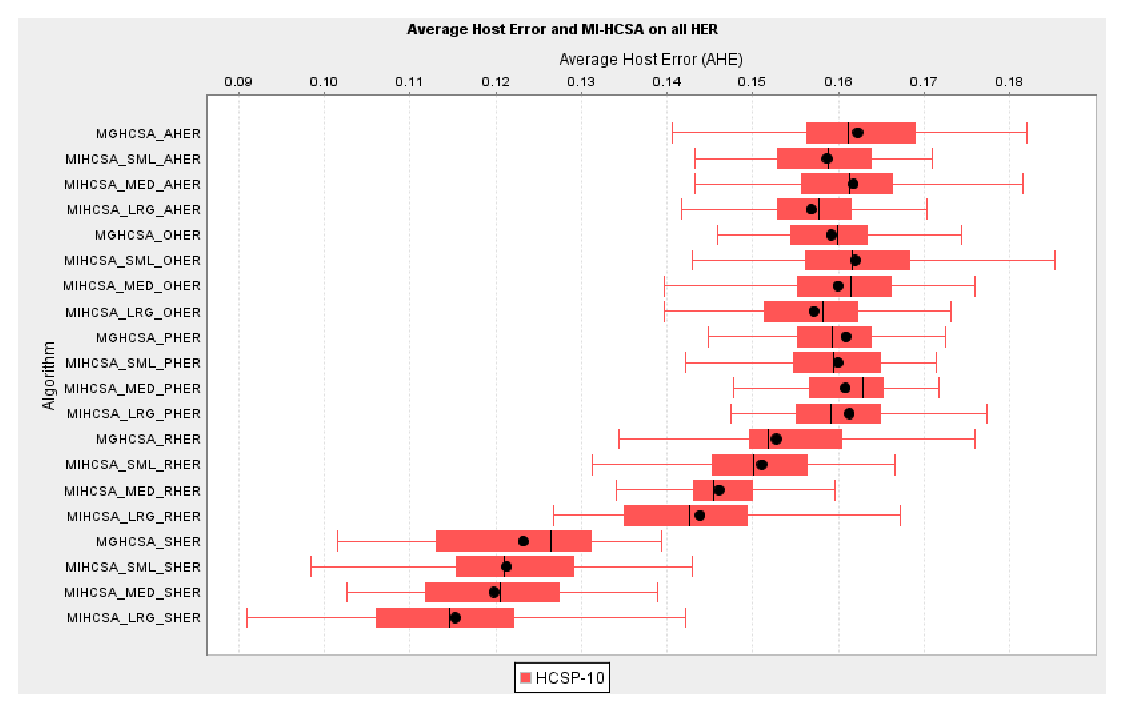
\includegraphics[scale=0.70]{Hosts/MI-HCSA-AHE}
	\caption{Box-and-whisker plot of Average Host Error (AHE) across all HER for the MI-HCSA study.}
	\label{fig:hosts:mihcsa:ahe:boxplot}
\end{figure}


%
% Analysis
%
\subsubsection{Analysis}
This section provides an analysis of the results from the empirical study into the MI-HCSA summarised in Table~\ref{tab:hosts:mihcsa:results}. These analyses exploit the trends and expectations outlined in Section~\ref{subsec:hosts:paradigm:realised:behaviours} regarding information dissemination between the hosts in the population.

%
% Generational Trends
%
\paragraph{Generational Trends}
% this section
This section compares and contrasts the minimal generational approach without sharing with the maternal immunity approach with inter-generational sharing. MG-HCSA is compared against MI-HCSA-L as it is expected to exhibit the largest effect of sharing and therefore difference to the minimal approach.
% system
From a system perspective MI-HCSA resulted in a generally population diversity and lower system error than MG-HCSA across all five of the exposure regimes. Interestingly this trend was not observed on the symmetric exposure regime, where no significant difference was observed.
% component
From a component perspective, maternal immunity generally achieved a lower Average Host Diversity and lower Average Host Error than the minimal approach. This was generally observed across the five HER's, except on SHER and PHER with regard to AHD and AHE respectively.
% trends
The results show a clear localisation effect with decreased error and increase in diversity at the system level, with the interesting side effect of decreased average error at the component level. The general lack of effect on the SHER suggests that the inter-generational sharing does not provide any benefit under such a strongly specialising exposure regime. The observations may be generalised to the following trends: 

\begin{enumerate}	
	\item Maternal immunity results in improved localisation compared to the minimal generational approach.
	\item Parent-Child inter-generational sharing provides an inter-generational localisation method resulting in highly-specialised hosts.
\end{enumerate}

%
% Maternal Immunity Size Trends
%
\paragraph{Maternal Immunity Size Trends}
% this section
This section considers the effect of varying the number of cells shared between the generations defined by different values for the $N_{maternalcells}$ user parameter.
% system
From a system perspective the results demonstrated an increase in effect with the number of transmitted maternal cells. Specifically, increase in $N_{maternalcells}$ resulted in an a increase in system diversity and decrease in system error. The effect was less pronounced with small sample sizes, typically with little significant difference between MG-HCSA and MI-HCSA-S as well as between MI-HCSA-S and MI-HCSA-M.
% component
From a component perspective the increase in the number of transmitted sampled cells resulted in relative increase in the effect as measured by decreases in Average Host Diversity and decreases in Average Host Error. The same general lack of significance was observed with small, medium and empty sample sizes.
% trends
The maternal cell size trend demonstrates that parent-child generational sharing promotes a strong localisation effect that increases with the amount of information communicated between the generations across the variety of exposure regimes. Importantly the effect is not apparent (significant) until a sufficiently large number of randomly selected cells are transmitted. The observations may be generalised to the following trends: 

\begin{enumerate}
	\item Localisation effect increases with the number of transmitted maternal cells.
	\item The number of cells must be of a sufficient size (50\%) for the effect to be consistently significant across the exposure regimes.
\end{enumerate}

%
% Conclusions
%
\subsubsection{Conclusions}
This section summarises the findings of the empirical study into the Maternal Immunity Host Clonal Selection Algorithm, in terms of the primitives that were the focus of the study and the expectations that motivated the study.

\begin{enumerate}
	% generational
	\item \emph{Generational}
	\begin{enumerate}
		\item The assessed specialisation of maternal immunity resulted in improved inter-generational specialisation than no inter-generational sharing.
	\end{enumerate}
	
	% parent child
	\item \emph{Parent-Child Sharing}
	\begin{enumerate}
		\item Maternal Immunity with parent-child sharing is an inter-generational localisation method.
		\item The concern of maternal immunity that sufficiently large sample sizes would result in homogeneous generations was confirmed to the benefit of the localisation effect resulting in reduced system and component-wise error.
	\end{enumerate}	
\end{enumerate}

% lifetime/generational
An important consideration not addressed is the differentiation from generational learning and lifetime learning. As mentioned in the method, the results were taken from the end of the run before a generational change, thus reflect generational learning over 9 generations of 100 epochs, and lifetime learning over 99 epochs in the final generation. Elaborative investigations may consider such a distinction and assess generational learning as the performance of the population before lifetime learning (at the epoch of creation), and lifetime learning before the generational change. When such a distinction is not made as in the case of this and the next empirical studies, the effects are still present, although aggregated (confounded) together.
% other approaches
The parent-child approach assessed is perhaps the simplest of such maternal immunity approaches. One may consider shifts in the cardinality between sharers in the previous generation and receivers in the next generation, with a clear relationship to the investigation into SI-HCSA and whether the results hold across generations. Two additional important questions that may motivate future work include (1) the consideration as to how much of the new generation must be seeded with maternal cells for the effect to be observed, and (2) the effect of positioning children in different parts of the antigenic environment (effecting the specialisation of children under the exposure regimes).

%
% Inherited Algorithms
%
\section{Generational Evolved Immunity}
\label{sec:hosts:generational:evolved}

%
% Generational Inheritance
%
\subsection{Generational Inheritance}
\label{sec:hosts:generational:evolved:theory}
% metaphor
The evolution of the immune system provides a inter-generational method for propagating functional aspects of the immune system based on lifetime performance.
% strategy
Unlike maternal immunity, evolution does not share acquired immune information directly in the form of cells, rather it shares it indirectly through selection and inheritance of the mechanisms that create and utilise those cells. 
% abstraction
An inherited generational algorithm requires a selection and reproduction mechanisms for hosts. The important differences in this specialisation of the generational algorithm is that a given host may contribute more or less than the other hosts in its generation. This is a realisation of natural selection, where a measure of the hosts in the population discriminates the reproductive fitness and genetic contribution to the next generation. The principle difference of this specialisation is the use of a genetic-basis for traits that effect hosts acquired immune system. The principle components of the inherited generational algorithm are defined as follows:

\begin{itemize}
	\item \emph{Selective Scheme}: A specialisation of the host selection scheme of the minimal generational algorithm that realises the principles of natural selection. A given hosts contribution to the subsequent generation is differentiated based on assessed fitness against an inherited trait that effects a hosts acquired immune system. 
	\item \emph{Genetic Basis}: A genetic code (genome) is used to define a trait of a hosts acquired immune system. This genetic code provides the basis of natural selection (differentiated reproductive success), and the medium for reproduction (genetic inheritance).
	\item \emph{Reproductive Scheme}: The reproductive scheme of the minimal generational population-based algorithm, that may take into account the broader considerations of asexual and sexual reproduction. Reproduction provides the basis for inheritance with regard to the genetic basis of the trait or traits that effect a hosts acquired immune system, and manipulations to that genetic representation in the form of genetic mutation and/or genetic recombination.
\end{itemize}

The reproductive scheme provides the mechanism for inheritance of the genetic basis of an acquired immune system trait. Reproduction provides a duplication of the parents genetic material which may be modified in minor ways by genetic mutation (likely a lower rate of mutation than that of hypermutation in the immune response). This introduces variations of the trait for natural selection to differentiate reproductive success. A property of the host populations acquired immune system is defined by a parameter or set of parameters, which is encoded in a genome. The genome is the basis for inheritance, and the expressed trait is the basis for host selection. For example, an inheritance mechanism may be defined that encodes information that defines the generation of \naive\ immune cells in a hosts acquired immune system. Unlike the maternal sharing scheme that directly reinforces the receptor configurations that are useful, an evolutionary algorithm indirectly reinforces receptor configurations in the generation of a hosts base repertoire, and ongoing \naive\ cells. This is a broader form of sharing that provides the flexibility for the selection mechanism and scope of the genetic basis for the trait to define the regions of `receptor configuration space' that are beneficial for a hosts untested acquired immune system to sample. The mechanism provides an interesting example that combines both genetic-based learning over generational time and somatic-based learning over a hosts lifetime. Therefore, this class of host algorithm facilitates \emph{learning at two scales}, specifically learning at the host-lifetime scale in somatic adaptations via clonal selection, and learning at the population-generation scale in genetic adaptations via natural selection. Examples of other traits that may be subjected to the pressures of evolution by natural selection include (1) the sensitivity of matching in the clonal selection algorithm (2) and the organisation and connectivity of tissue types in the lymphoid tissue algorithm. In addition to opening up parameterised models in the framework to the process of evolution via natural selection (generational learning), the minimal natural selection algorithm provides a connection of the host-level of the acquired immune system framework with the field of genetic algorithms.

\begin{algorithm}[htp]
  \SetLine
  \SetKwData{Pop}{P}
  \SetKwFunction{HostError}{HostError}
  \SetKwFunction{BiasedRouletteWheelSelection}{BiasedRouletteWheelSelection}
  \SetKwFunction{Crossover}{Crossover}
  \SetKwFunction{Mutate}{Mutate}  
  
  \KwIn{\Pop, $P_{mutation}$, $P_{crossover}$}
	\KwOut{$P\prime$} 		
	
	$P\prime \leftarrow$0\;			
	% assess the current population	
	\ForEach{$H_i \in$ \Pop}
	{
		$H_iFitness \leftarrow $ \HostError{$H_i$}\;
	}
	% select the parents
	$P_{parents} \leftarrow$0\;
	\For{i$\leftarrow$0 \KwTo $N_{hosts}$}
	{
		$H_i \leftarrow$ \BiasedRouletteWheelSelection{\Pop}\;
		$P_{parents} \leftarrow H_i$\;
	}		
	% create the children from the parents
	\ForEach{$H_i$, $H_{i+1} \in P_{parents}$}
	{
		$H_ichild_1 \leftarrow $ \Crossover{$H_i$, $H_{i+1}$, $P_{crossover}$}\;
		$P\prime \leftarrow H_ichild_1$\;
		$H_ichild_2 \leftarrow $ \Crossover{$H_i$, $H_{i+1}$, $P_{crossover}$}\;
		$P\prime \leftarrow H_ichild_2$\;
	}
	% mutation
	\ForEach{$H\prime_i \in P\prime$}
	{
		\Mutate{$H\prime_i$, $P_{mutation}$}\;
	}	
	\Return{$P\prime$}\;
	\caption{CreatePopulation for the Evolved Immunity Clonal Selection.}
	\label{alg:hosts:algorithms:eihcsa}
\end{algorithm}

% algorithm
The \emph{Evolved Immunity Host Clonal Selection Algorithm (EI-HCSA)} is defined as a specialisation of the Generational Host Clonal Selection Algorithm (defined in Algorithm~\ref{alg:hosts:algorithms:ghcsa}) that uses a genetic basis, host selection and host reproduction schemes as defined in the $CreatePopulation$ operation in Algorithm~\ref{alg:hosts:algorithms:eihcsa}. The $P_{mutation}$ parameter defines the probability of mutating a component in the hosts genetic representation during reproduction, and $P_{crossover}$ defines the probability of creating two new host from a cross of two parental hosts genetic basis. The reproduction scheme is a rudimentary realisation of the classical genetic algorithm (discussed in Section~\ref{subsec:cs:related:ec}) for a hosts initial repertoire.

%
% Empirical Study
%
\subsection{Evolved Immunity Empirical Study}
\label{sec:hosts:generational:evolved:study}

%
% Aim
%
\subsubsection{Aim}
The aim of this empirical study is to investigate the Evolved Immunity Host Clonal Selection Algorithm in the context of the information dissemination and localisation capabilities as compared to the Minimal Generational Host Clonal Selection Algorithm under a variety of host exposure regimes. Toward this end, the study had the following goals:

\begin{enumerate}
	\item Compare and contrasted generational clonal selection with and without an inherited initial repertoire.
	\item Investigate the localisation and/or dissemination properties of inter-generational inheritance.
\end{enumerate}


%
% Method
%
\subsubsection{Method}

%
% Algorithms
%
\paragraph{Algorithms}
The study considered the Minimal Generational Host Clonal Selection Algorithm (MG-HCSA) and the Evolved Immunity Host Clonal Selection Algorithm (EI-HCSA).
% MG-HCSA
MG-HCSA is a specialisation of the HCSA defined in Algorithm~\ref{alg:hosts:algorithms:ghcsa}, that was configured with $N_{hosts}=10$. Each $H$ was configured with a single tissue ($N_{tissues}=1$) that was an instance of the RCCSA defined in Algorithm~\ref{alg:cells:realisation:algorithms:rccsa:exposure}, with the configuration $N_{cells}=50$, $N_{selection}=1$, and $N_{clones}=5$. The $CreatePopulation$ operation for the MG-HCSA was realised as the creation of a new population of hosts each generational change as defined in Algorithm~\ref{alg:hosts:algorithms:ghcsa:mghcsa}, and the epoch generational change condition defined in Equation~\ref{eq:hosts:algorithms:generationalchange} with $N_{genepochs}=100$.
% EI-HCSA
The MI-HCSA with assessed with the evolutionary specialisation of the $CreatePopulation$ operation defined in Algorithm~\ref{alg:hosts:algorithms:eihcsa}. Host fitness was assigned using the AHE measure. The probability of crossover was fixed at 0.90 (90\%) per host-pair creation. The mutation duration host creation was $\frac{1}{192}$ bits which is one mutation cell or 50 mutations per population creation ($\frac{50}{9600}$ bits). 

%
% Problems
%
\paragraph{Problems}
The same Habitat Colour Space Problem and Host Exposure Regimes were used as was defined for the THCSA Empirical Study in Section~\ref{sec:hosts:population:elicited:study}.

%
% Experiment
%
\paragraph{Experiment}
The same experimental setup was used as was defined for the MI-HCSA empirical study in Section~\ref{sec:hosts:generational:maternal:study}, expect the maximum number of epochs on the EOSC stop condition was increased from 999 to 9999. This configuration change was made such that the final measures recorded reflected the state of the system after 100 generations of 100 epochs before the last generational change at one hundredth generation.

%
% Results
%
\subsubsection{Results}
Table~\ref{tab:hosts:eihcsa:results} in Appendix \ref{appendix:results:hosts:evolved} provides a summary of results for each algorithm-problem combination including the mean ($\bar{x}$) and standard deviation ($\sigma$) of collected measure values.  Box-and-whisker plots are provided in which the results for each algorithm are aggregated across all HER for a each measure. Figure~\ref{fig:hosts:eihcsa:pd:boxplot} shows PD, Figure~\ref{fig:hosts:eihcsa:pe:boxplot} shows PE, Figure~\ref{fig:hosts:eihcsa:ahd:boxplot} shows AHD, and Figure~\ref{fig:hosts:eihcsa:ahe:boxplot} shows AHE.

\begin{figure}[htp]
	\centering
		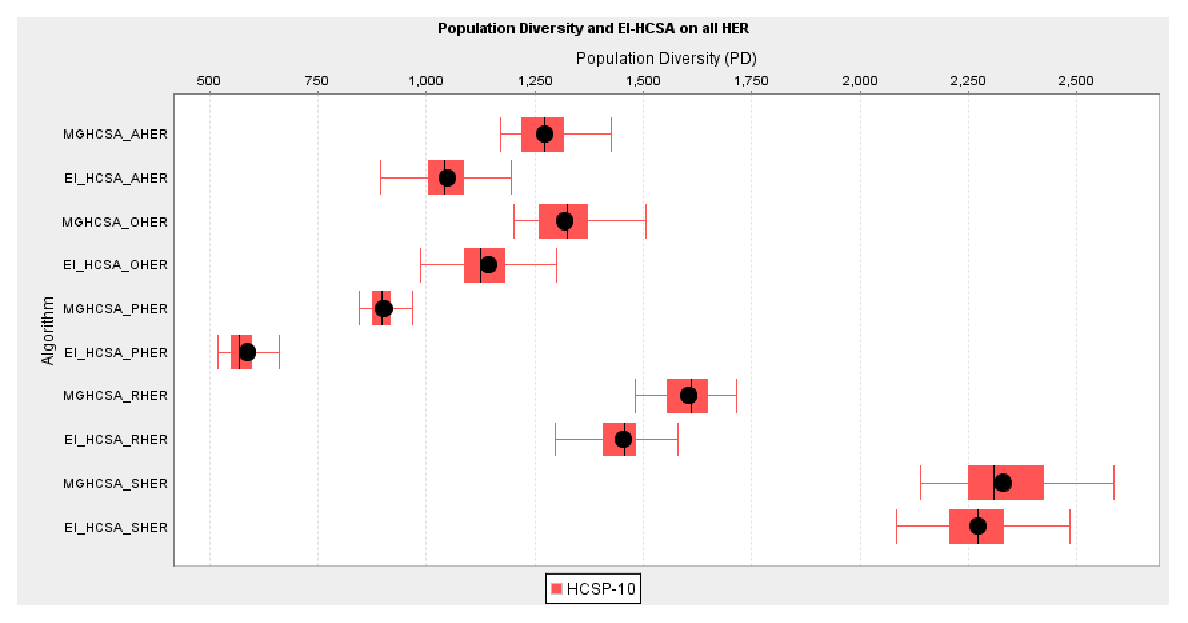
\includegraphics[scale=0.70]{Hosts/EI-HCSA-PD}
	\caption{Box-and-whisker plot of Population Diversity (PD) across all HER for the EI-HCSA study.}
	\label{fig:hosts:eihcsa:pd:boxplot}
\end{figure}

\begin{figure}[htp]
	\centering
		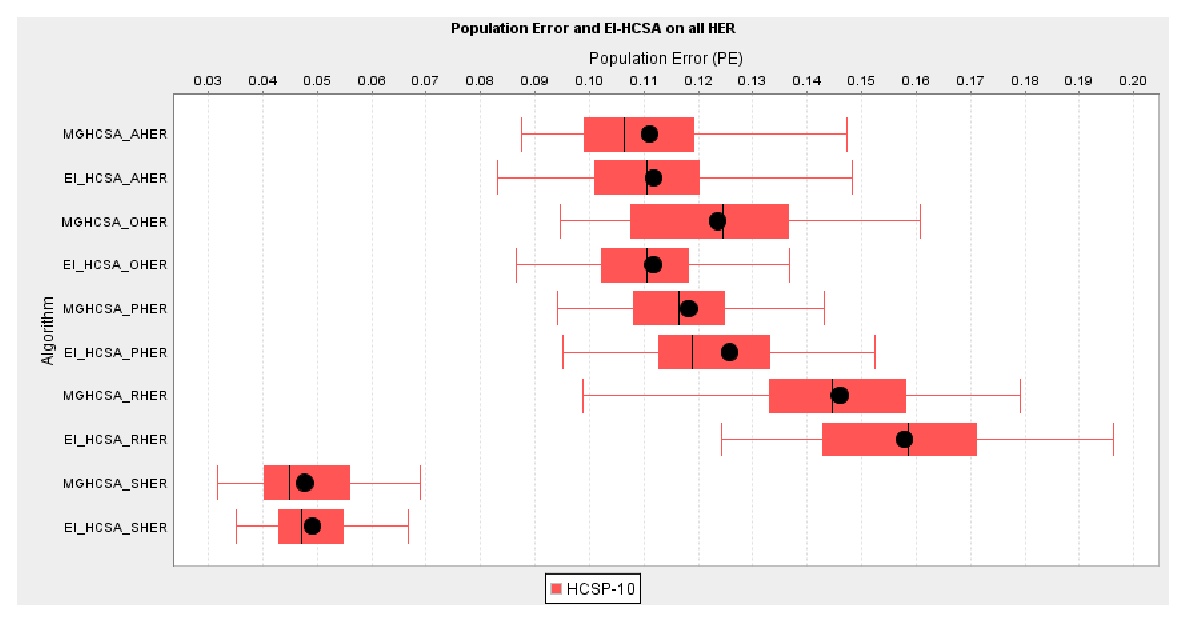
\includegraphics[scale=0.70]{Hosts/EI-HCSA-PE}
	\caption{Box-and-whisker plot of Population Error (PE) across all HER for the EI-HCSA study.}
	\label{fig:hosts:eihcsa:pe:boxplot}
\end{figure}

\begin{figure}[htp]
	\centering
		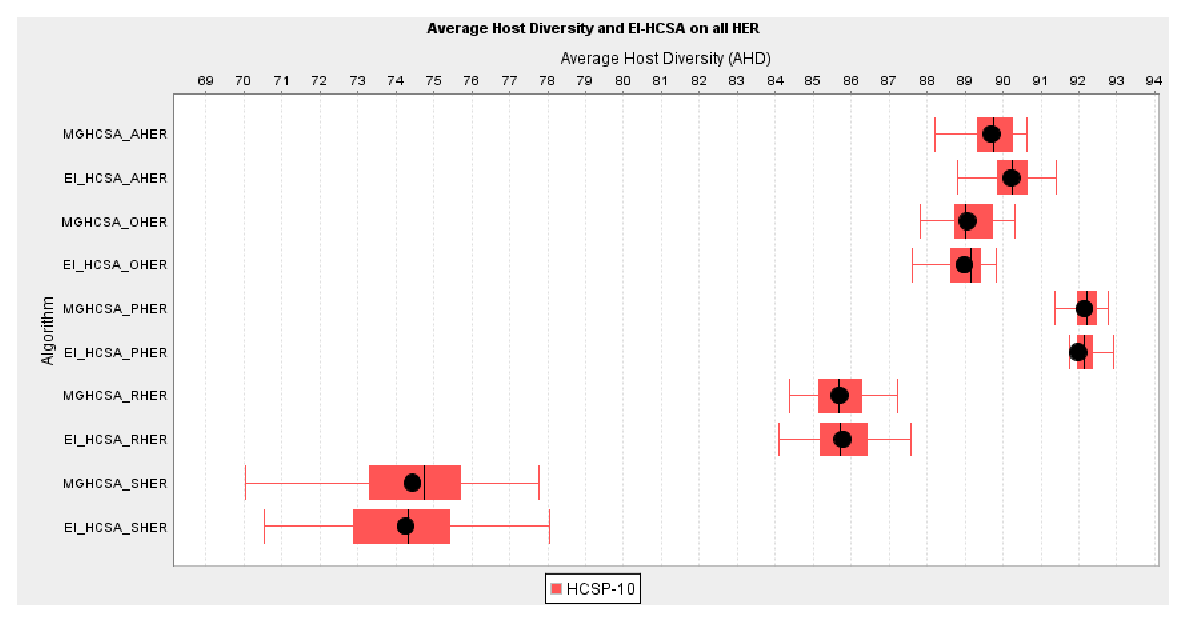
\includegraphics[scale=0.70]{Hosts/EI-HCSA-AHD}
	\caption{Box-and-whisker plot of Average Host Diversity (AHD) across all HER for the EI-HCSA study.}
	\label{fig:hosts:eihcsa:ahd:boxplot}
\end{figure}

\begin{figure}[htp]
	\centering
		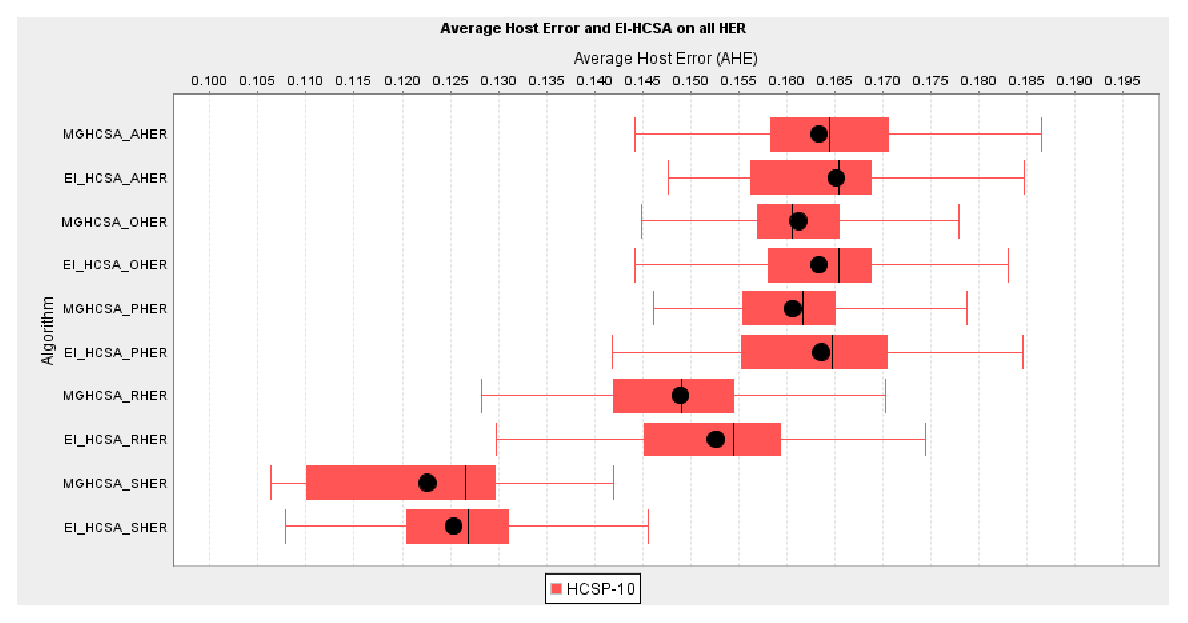
\includegraphics[scale=0.70]{Hosts/EI-HCSA-AHE}
	\caption{Box-and-whisker plot of Average Host Error (AHE) across all HER for the EI-HCSA study.}
	\label{fig:hosts:eihcsa:ahe:boxplot}
\end{figure}

%
% Analysis
%
\subsubsection{Analysis}
This section provides an analysis of the results from the empirical study into the MI-HCSA summarised in Table~\ref{tab:hosts:eihcsa:results}. These analyses exploit the trends and expectations outlined in Section~\ref{subsec:hosts:paradigm:realised:behaviours} regarding information dissemination between the hosts in the population.

%
% Generational Trends
%
\paragraph{Generational Trends}
% this section
This section compares and contrasts the evolved immunity algorithm against the minimal generational approach. 
% system
From a system perspective the evolved immunity algorithm generally exhibited a decrease in population diversity compared to the minimal generational algorithm, although the trend was not significant on the symmetric exposure regime. A difference in population error between the approaches was only significant on OHER and RHER, where a decrease and increase were observed respectively. 
% component
From a component perspective there was practically no significant difference between EI-HCSA and MG-HCSA with regard to Average Host Diversity and Error, other than a small increase in diversity in the evolved approach on AHER.
% trends
The results demonstrate little significant difference between the two approaches other than a general decrease in population diversity and some changes to system error. The change in population diversity provides confirmation that the evolutionary mechanisms were providing a convergence effect, resulting in increased homogeneity between the hosts in the population. 

\begin{enumerate}
	\item Generally there is little difference between inherited immunity and independent generations for the chosen configuration.
	\item Decreased population diversity may suggest at an evolutionary effect that promotes a a population of homogeneous genetic material (evolutionary convergence). 
\end{enumerate}

%
% Conclusions
%
\subsubsection{Conclusions}
% reasons for bad performance
Two considerations that may have resulted in the lack of significance between the two approaches include (1) the amount of evolution permitted given the complexity of the problem, and (2) the noisiness of the fitness function. In the first case the configuration permitted 100 evolutionary generations each with 100 epochs providing a testing ground for the host genetic basis. Given that this genetic basis consisted of 9600 bits, it is more than likely that an increase in the number of generations (such as a factor of 10 or 100) would result in a significantly increased evolutionary effect toward a homogeneous host genetic footprint. In the second case, the objective function used (genetic system competence via host error) may have proven too noisy given the reduced amount of interaction with the problem (100 environment exposures). In addition, such an objective, although desirable may have been convoluted by the asymmetry of information exposure by some of the exposure regimes providing a potentially second level of noise. This may be tested by again increasing the number of generations and/or the number of epochs per generation, as well as testing on simpler symmetrical and deterministic exposure regimes.

% extension
The proposed inherited immunity approach aligned with the general progression in complexity with the proposed host clonal selection algorithms, although in the context of the potential of combining abstractions of evolution and the acquired immune system was very simplistic. The principle of combining the approaches begs for elaborated investigation.

%
% Summary
% A summary of what the chapter contains, A description of how this leads into the next chapter
%
\section{Chapter Summary}
\label{sec:hosts:summary}

%
% Paradigm Review
%
\subsection{Paradigm Review}
% principles of the paradigm
The \emph{Host Clonal Selection Paradigm (HCSP)} was defined as the investigation of the Tissue and Cellular Clonal Selection Paradigms as constrained by (1) multiple holistic immune systems called \emph{Hosts} and their interactions, and (2) the concerns of regimes of discrete host exposures of information from an antigenic environment called \emph{Host Exposure Regimes (HER)}.
% metaphor
The paradigm exploits the metaphor of a collective of holistic acquired immune systems called a \emph{Population} and the turn-over of populations called \emph{Generations}. Intra-population communication is mediated by the hosts themselves as well as by pathogen that may spread through host-to-host contact. Intra-generational communication is mediated by parent-progeny relationships both explicitly and implicitly via an evolutionary process.
% abstraction
The principle information processing interest of the paradigm as gleamed from the metaphor are the information management strategies that may be employed to address the known and unknown regularities and irregularities in an antigenic \emph{Environment} of information called an \emph{Habitat Antigenic Exposure Problem (HAEP)}. The concern of such strategies is the effective intra-population and intra-generational dissemination of information between spatially isolated hosts and temporally isolated populations toward improved host-wise and population-wise capabilities whilst maintaining the intrinsic localisation of the adaptive units independence. 

%
% Principles and Findings
%
\subsection{Principles and Findings}
The following summarises the important principles and findings from the definition and investigations into the Host Clonal Selection Paradigm:

\paragraph{General Principles}
		\begin{enumerate}
			\item \emph{Host-mediated dissemination}: Unlike the Tissue Paradigm that provides a natural intra-component communication channel, the focus of the Host Paradigm is the development of information strategies to promote the controlled dissemination of acquired information toward improved population capability.
			\item \emph{Strategies based on host-level immunology}: Population immunology such as immunisation and evolutionary immunology inspire information strategies for acquiring, localisation, and disseminating information in an unknown environment as the survival of a population of organisms with immune systems rely on such strategies for survival.
		\end{enumerate}


\paragraph{Specific Findings}
		\begin{enumerate}
			\item \emph{Transmission}: Elicited immunity via pathogen transmission exhibits an information dissemination effect on exposure regimes with an asymmetric information distribution with little difference in effect whether immunity is elicited by random-pairing based pathogen transmission or one-to-many based vaccination.
			\item \emph{Shared Immunity}: Shared immunity via effector transmission results in a disruptive effect at the system and component level with large numbers of shared effectors, which is minimised with small scale intra-population sharing maximises the dissemination effect at the component level.
			\item \emph{Maternal Immunity}: Generational transmission via maternal immunity in parent-child relationships results in an inter-generational localisation method exploiting the generational homogeneity promoted by the mechanism.
			\item \emph{Evolved Immunity}: Evolved immunity via generational inheritance demonstrated comparatively little difference over generational restarts other than a suggestion at evolutionary convergence toward a consistent genetic footprint, suggesting at the potential of the under investigated combination of generational learning via evolution with lifetime learning via the acquired immune system.
		\end{enumerate}

%
% Integration
%
\subsection{Integration}
The Tissue Clonal Selection Paradigm in Chapter \ref{chap:tissues} took the Cellular Paradigm from Chapter \ref{chap:cells} for granted, using it as a principle component in the Tissue Clonal Selection Algorithm, focusing on how different decentralised information management strategies effected the organisation acquisition and use of information under different information exposure regimes. In the same manner the Host Paradigm in this chapter took the Tissue Paradigm for granted, subsuming the scope of inter-tissue interaction concerns and using the system in its entirety as a principle component (Host) in a the Host Clonal Selection Algorithm. The population provided the first abstraction of multiple hosts, concerned with decentralised information dissemination strategies, whereas the generational-population abstraction subsumed the concerns of a given population, highlighting the related but different concerns of inter-generational decentralised information dissemination strategies. These two abstractions represent the pinnacle in the exploration of the clonal selection paradigm presented in this work. The following chapter considers the aggregation of all three paradigms (cellular, tissue, and host) in a unifying framework that provides both explanatory power for presented algorithms, as well as predictive power in highlighting unrealised algorithms and other facets of the considered abstractions.
% application
The abstract host paradigm is grounded in Chapter~\ref{chap:iidle} in the context of two general problem domains, highlighting the potential benefits the tissue algorithms provide over the cellular clonal selection algorithms.


% EOF